\section{Istruzioni per l'uso}
\subsection{Requisiti di sistema}
Essendo un applicativo web, i requisti necessari al funzionamento di \emph{Premi} si limitano ai seguenti:
\begin{itemize}
\item Browser$_G$ che supporti la tecnologia HTML5$_G$;
\item Connessione ad Internet;
\item Javascript$_G$ abilitato sul proprio browser$_G$.
\end{itemize}

\subsection{Guida all'installazione}
*************Guida all'installazione di Meteor ecc..********************

\subsection{Primo accesso}
Al primo accesso il sistema richiede l'autenticazione dell'utente qualora fosse già registrato al sistema, altrimenti fornisce la possibilità di creare un nuovo account.
\begin{figure}[h]
\begin{center}
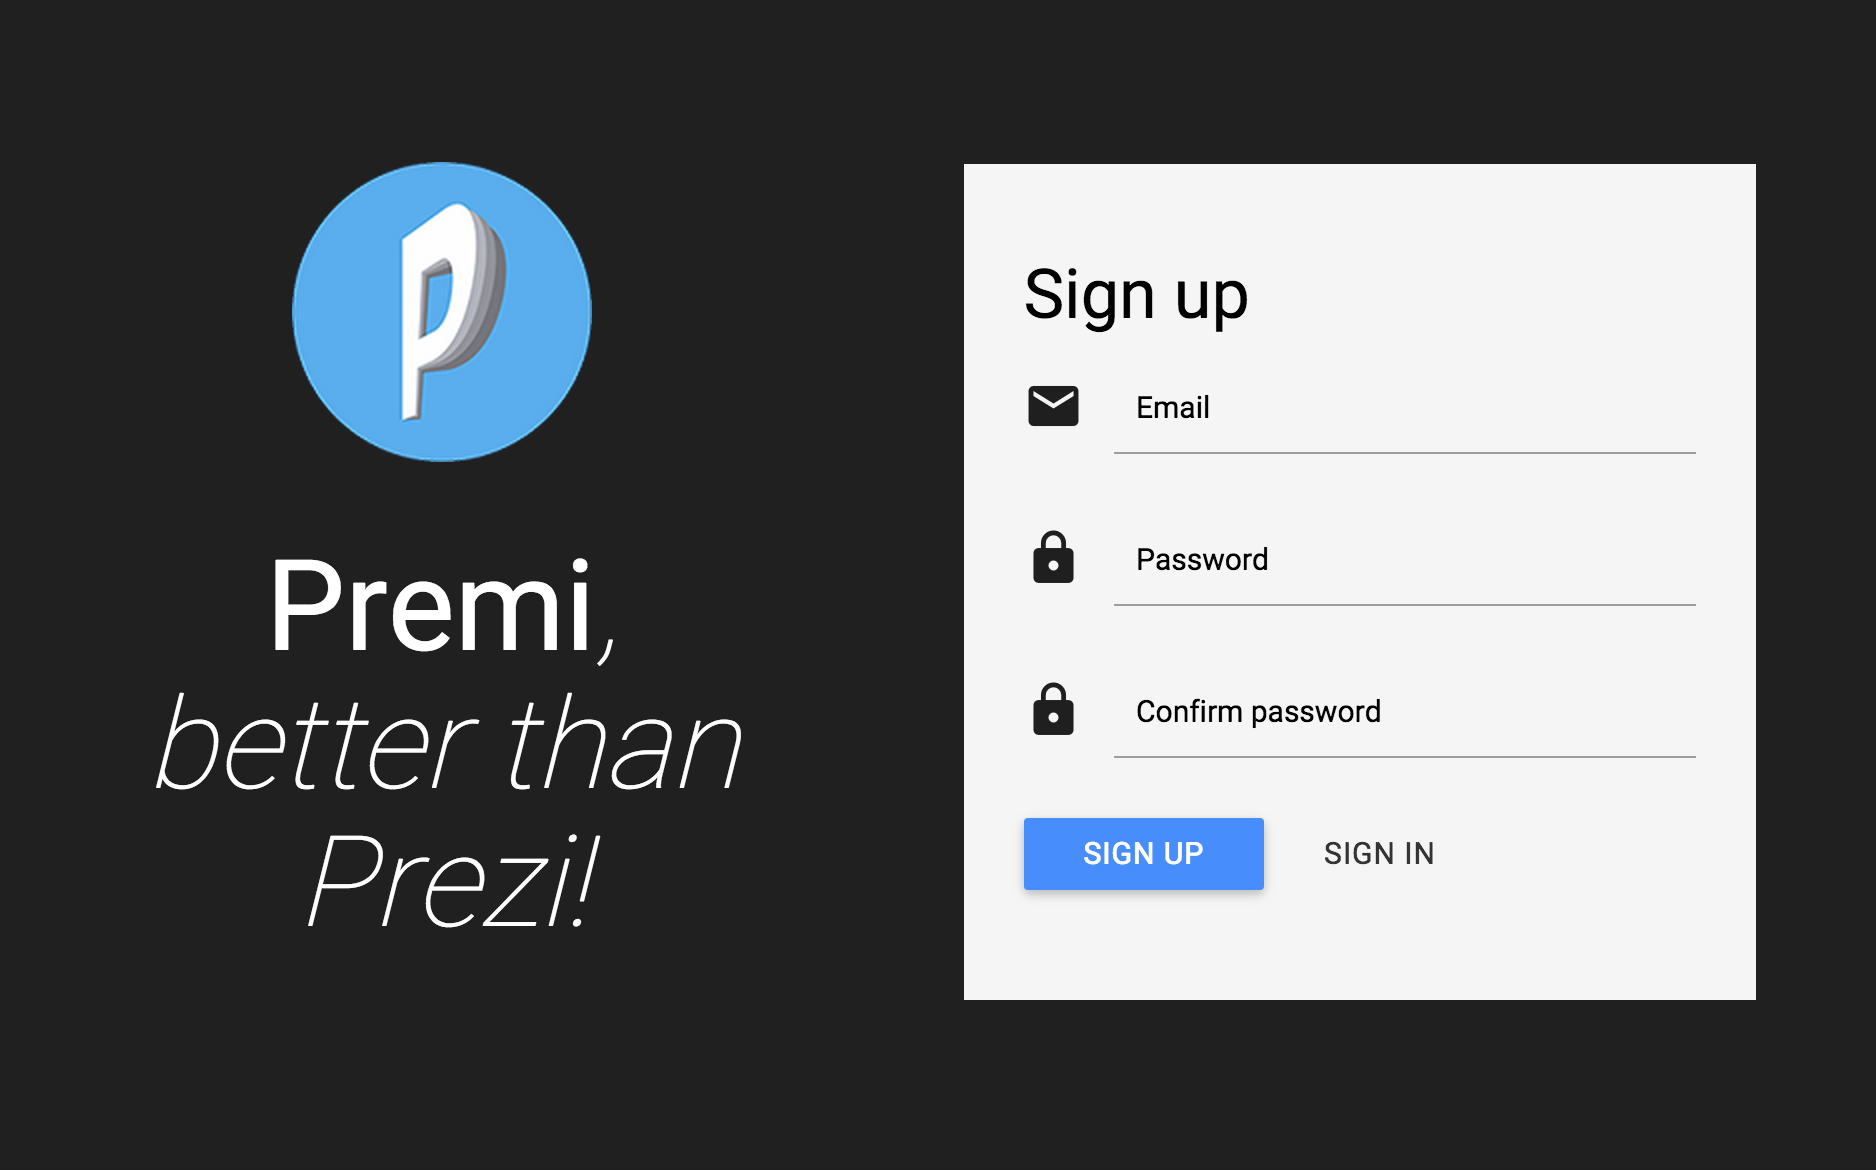
\includegraphics[scale=0.4]{img/signup.png}
\caption{Form di registrazione.}
\end{center}
\end{figure}

Per la creazione di un nuovo account i dati da inserire sono soggetti ad alcuni vincoli:
\begin{itemize}
\item Indirizzo email: deve essere un indirizzo valido;
\item Password: composta da almeno n. caratteri;
\item Conferma password: deve coincidere con il campo password precedente.
\end{itemize}
Per confermare la registrazione premere sul tasto "SIGN UP".
\begin{quote}
\textbf{Nota:} si potrebbero ricevere degli avvisi che notificano l'errato inserimento dei dati richiesti.
\end{quote}
Una volta completata la registrazione è necessario autenticarsi al sistema:
\begin{figure}[h]
\begin{center}
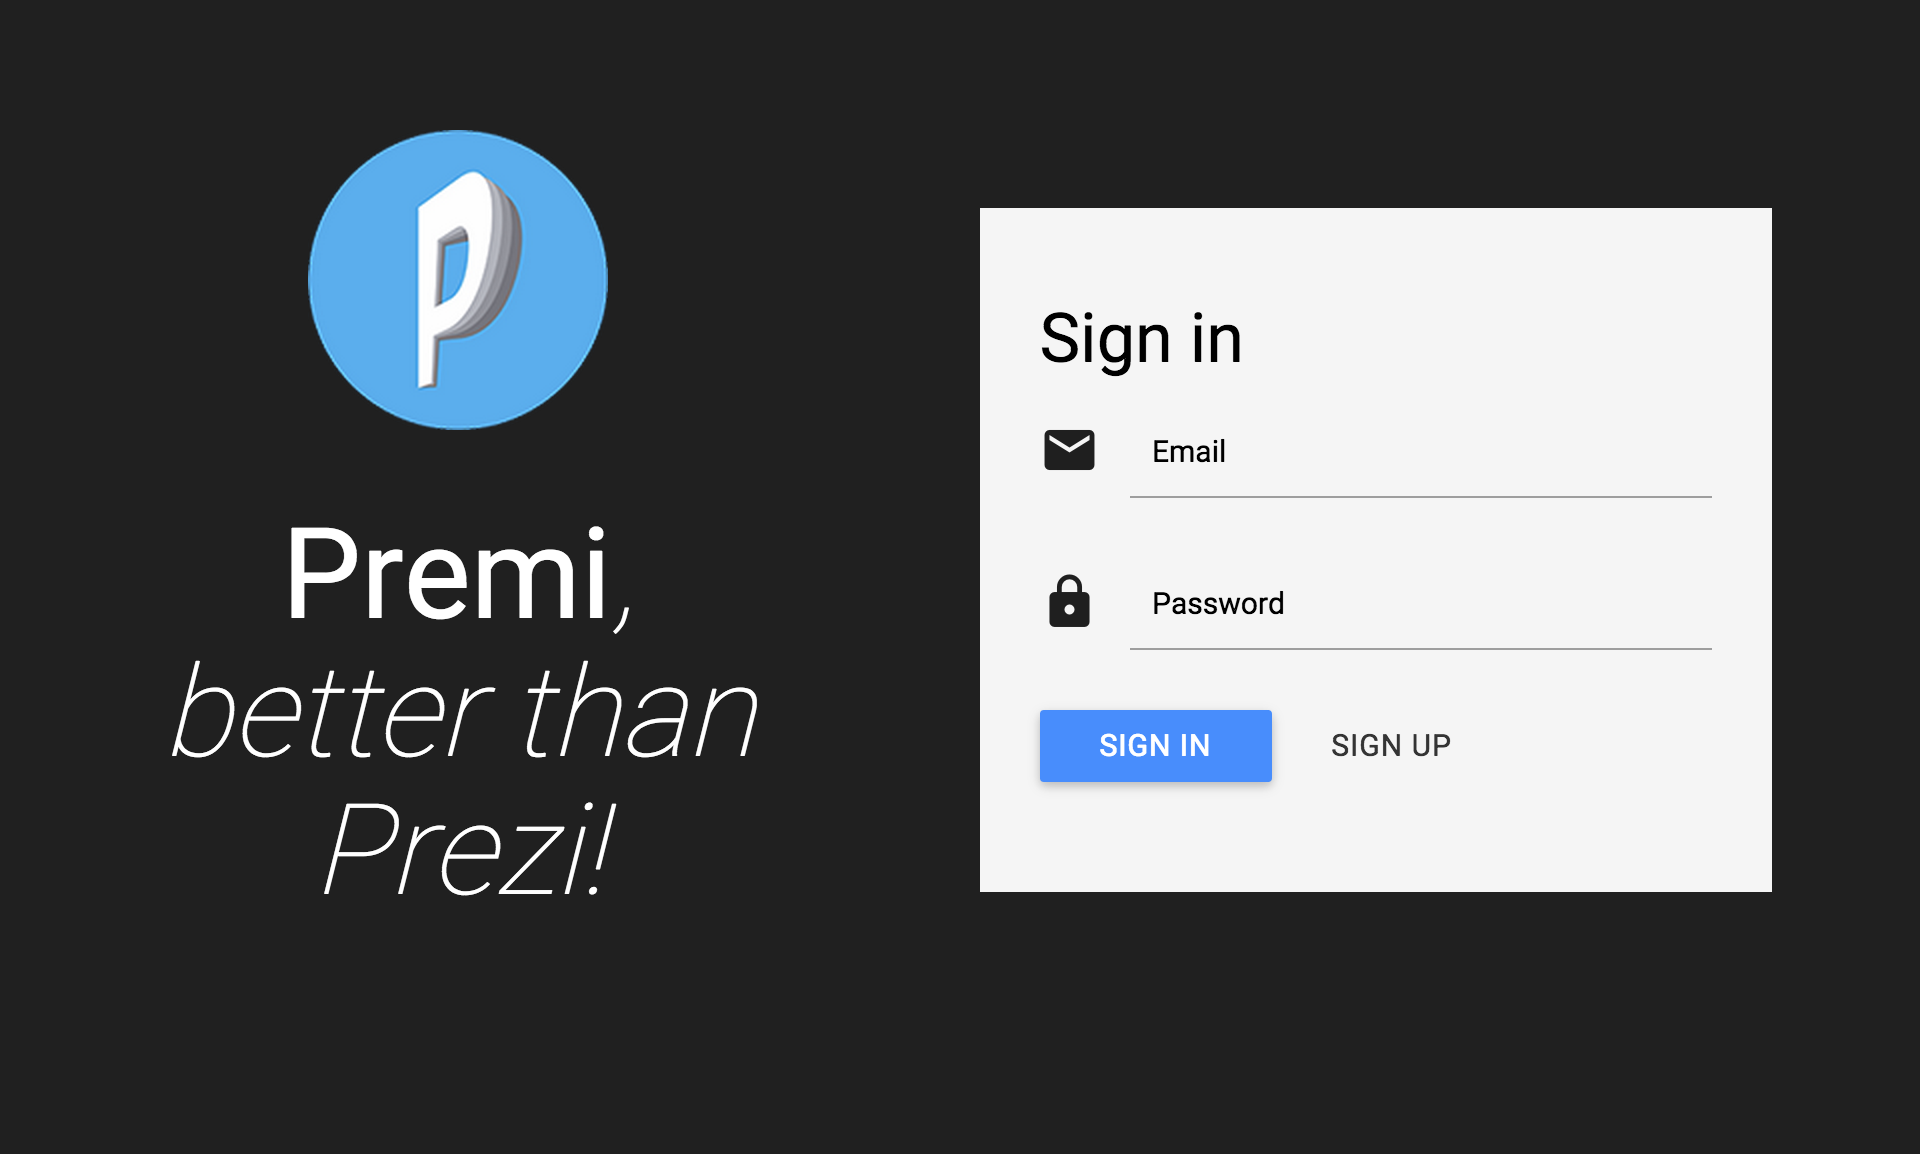
\includegraphics[scale=0.4]{img/signin.png}
\caption{Autenticazione al sistema.}
\end{center}
\end{figure}

\newpage
\subsection{Pannello di controllo dell'utente}
Una volta autenticati al sistema si accede al proprio pannello di controllo, all'interno del quale saranno visibili tutte le presentazioni finora create.
\begin{figure}[h]
\begin{center}
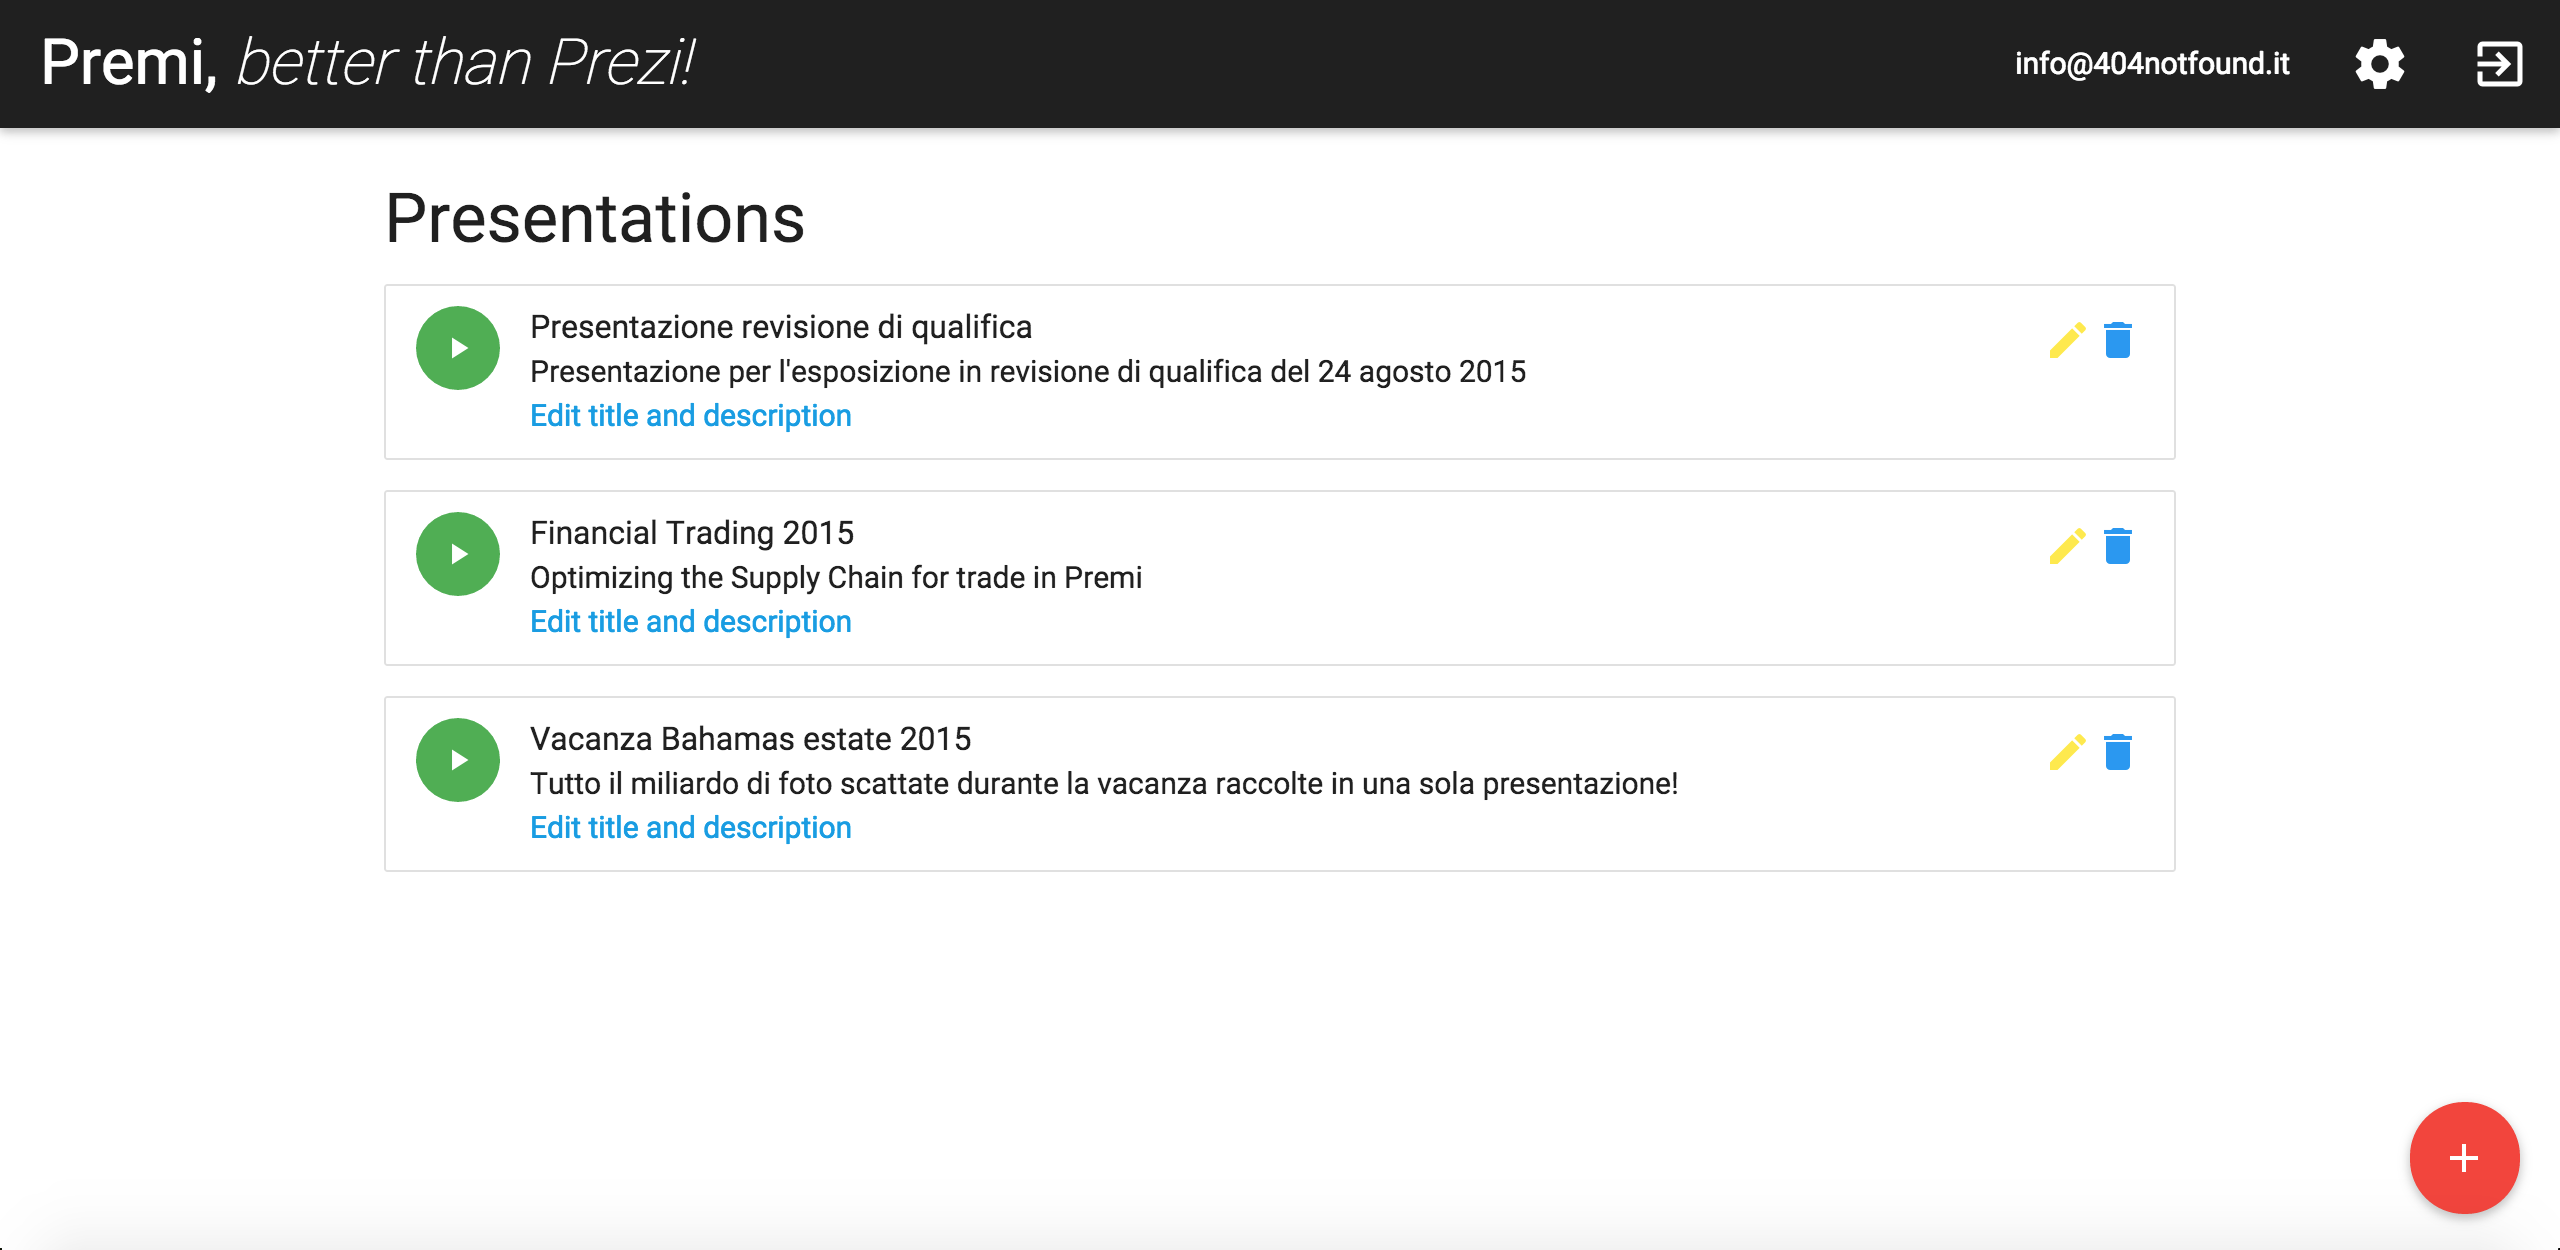
\includegraphics[scale=0.35]{img/dashboard.png}
\caption{Pannello di controllo utente.}
\end{center}
\end{figure}

Comandi:\\ \\
\begin{tabular}{ c l }
\parbox[c]{2em}{
\includegraphics[scale=0.6]{img/gear.png}} & Permette la modifica dei dati dell'account;\\
\parbox[c]{2em}{
\includegraphics[scale=0.6]{img/quit.png}} & Consente all'utente di disconnettersi dal sistema;\\
\parbox[c]{2em}{
\includegraphics[scale=0.4]{img/add.png}} & Permette la creazione di una nuova presentazione.\\
\end{tabular}

\newpage
\subsection{Creare una nuova presentazione}
\begin{figure}[h]
\begin{center}
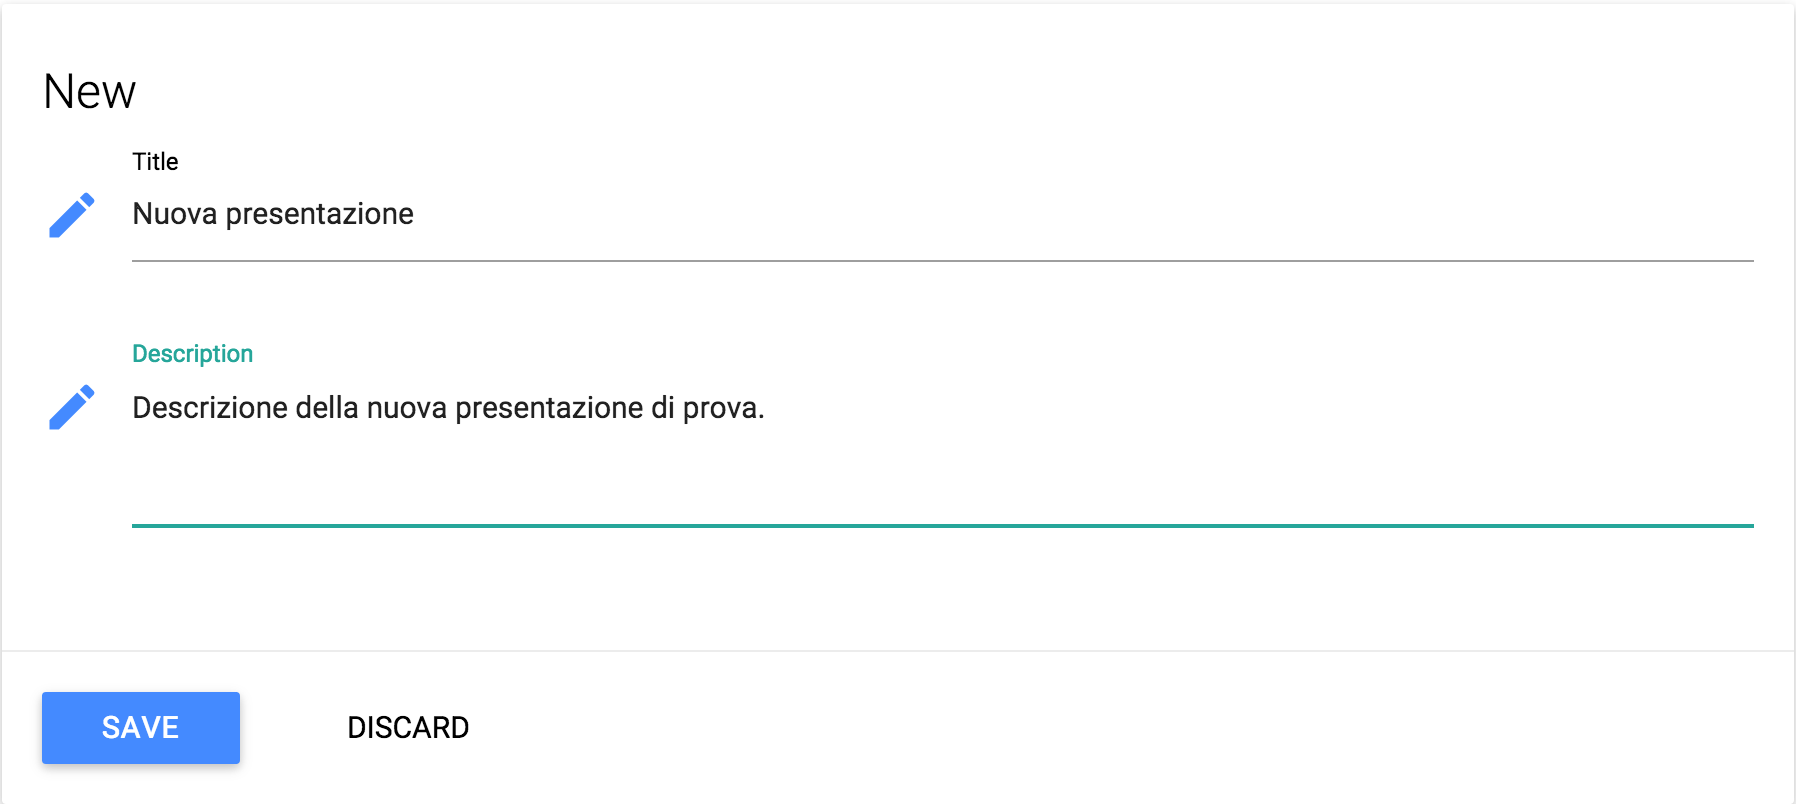
\includegraphics[scale=0.4]{img/new_pres.png}
\caption{Creazione nuova presentazione.}
\end{center}
\end{figure}

Per creare una nuova presentazione sarà sufficiente inserire il titolo e una descrizione, come visualizzato nella figura 4.
Una volta creata la presentazione questa verrà automaticamente aggiunta all'elenco delle presentazioni personali.
\begin{figure}[h]
\begin{center}
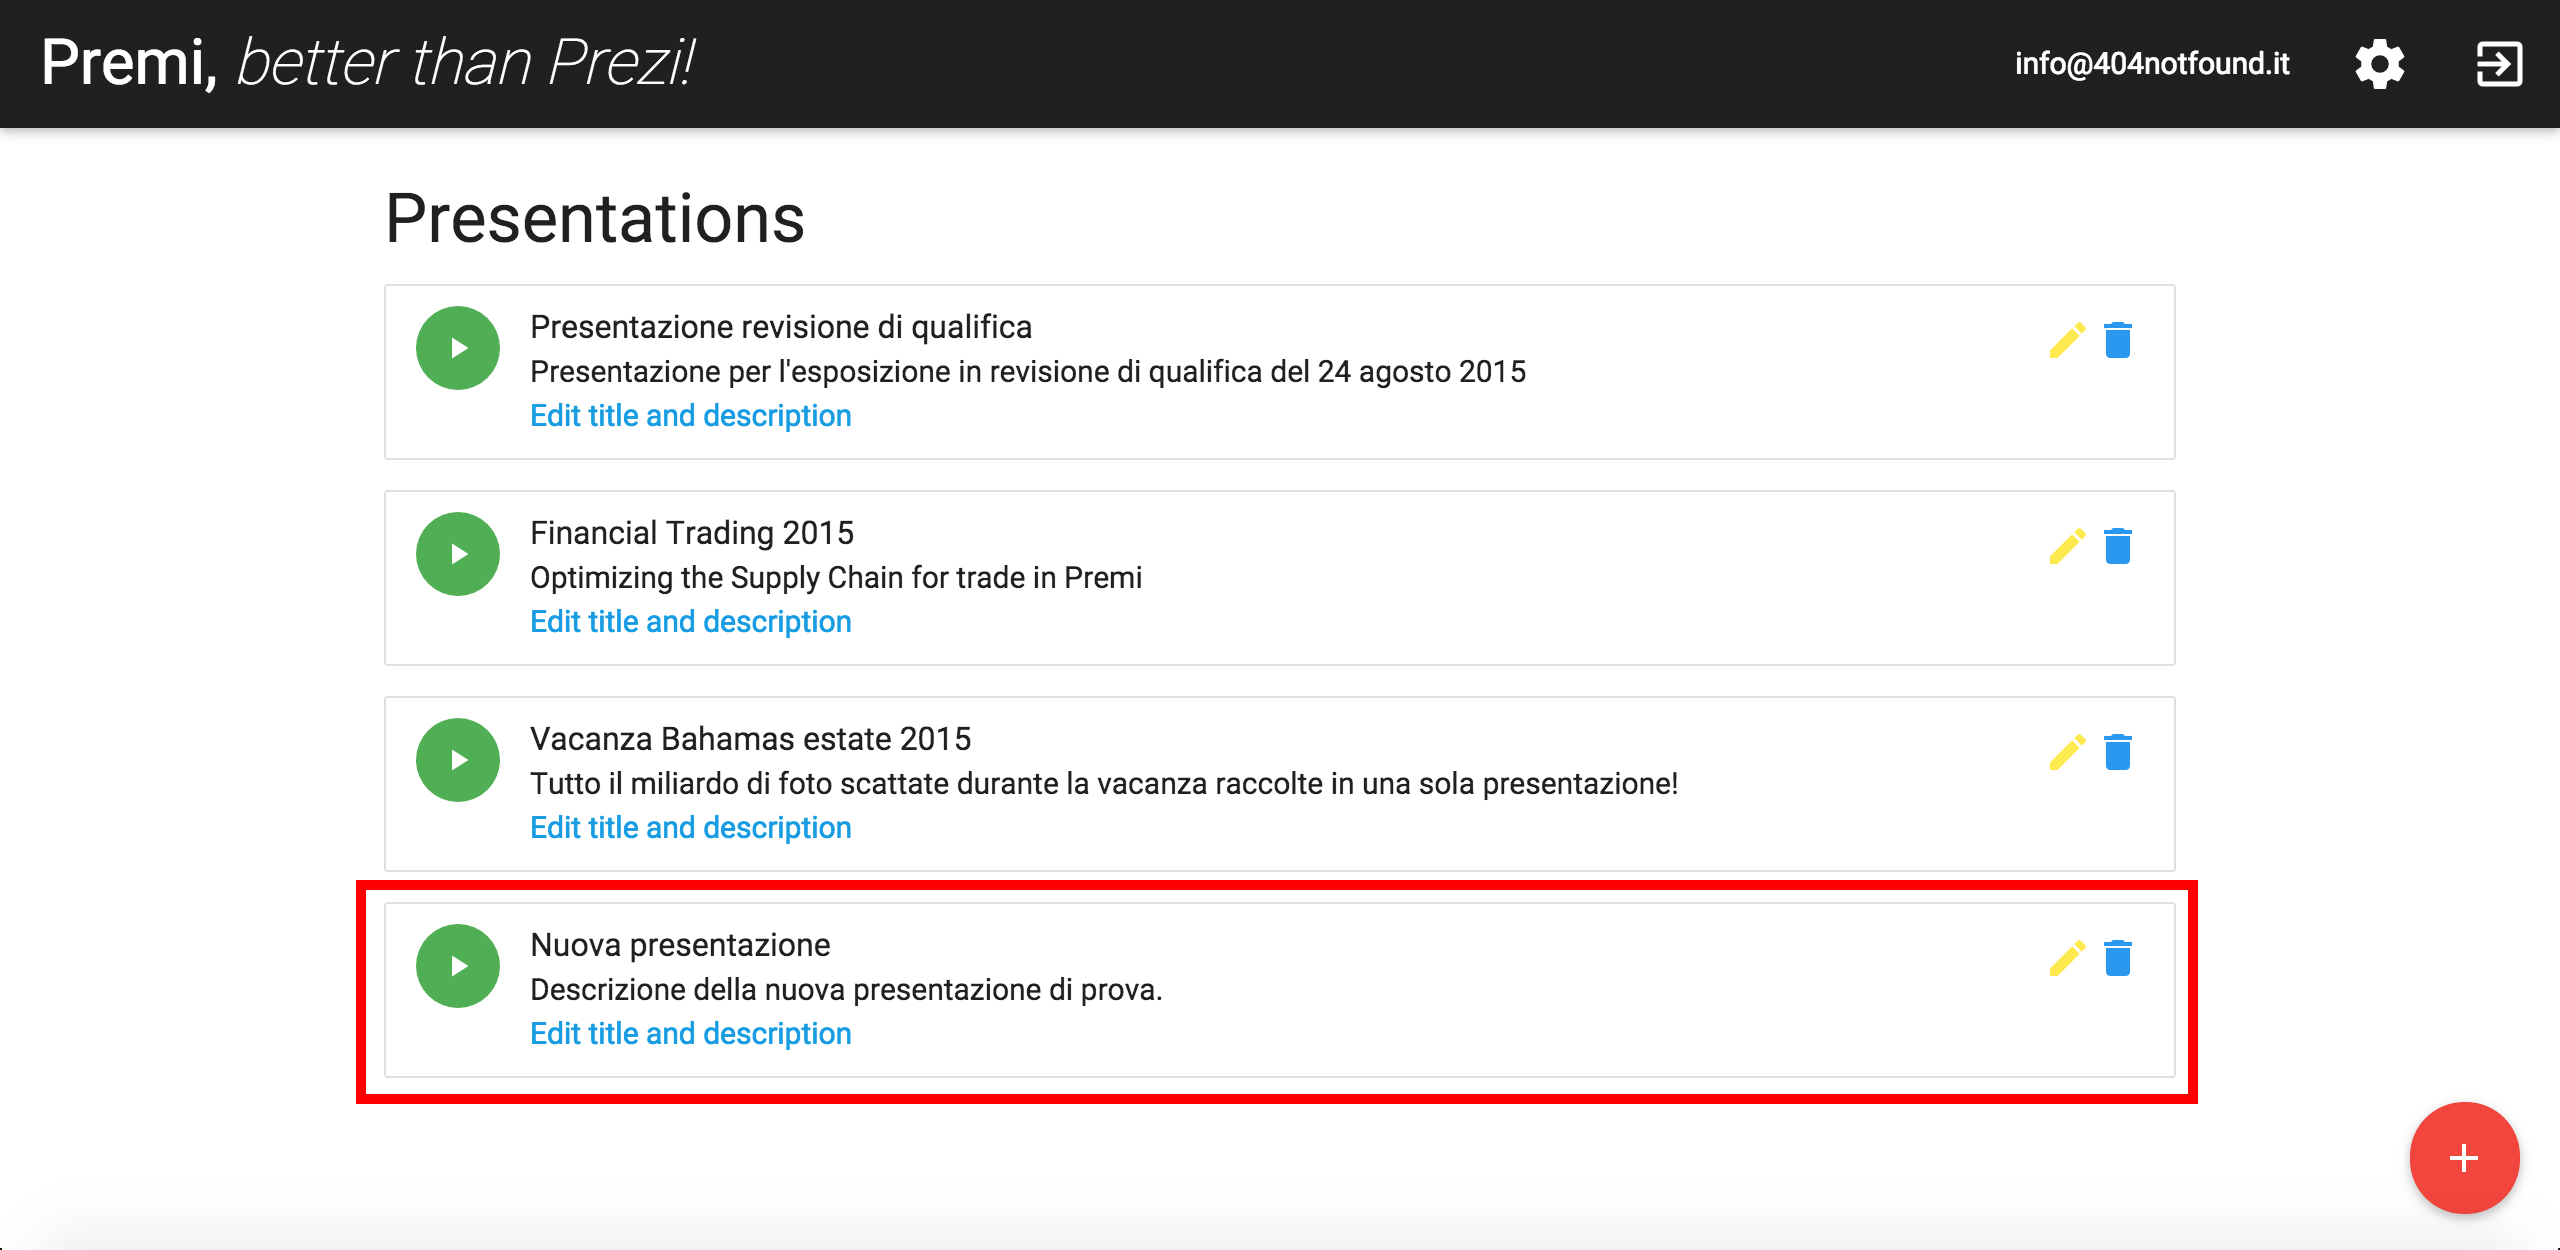
\includegraphics[scale=0.35]{img/list.png}
\caption{Lista presentazioni.}
\end{center}
\end{figure}

Ogni presentazione ha a disposizione tre azioni:\\

\begin{tabular}{ c l }
\parbox[c]{2em}{
\includegraphics[scale=0.4]{img/play.png}} & Avvia la presentazione;\\
\parbox[c]{2em}{
\includegraphics[scale=0.7]{img/edit.png}} & Modifica la presentazione. Apre la modalità editor$_G$;\\
\parbox[c]{2em}{
\includegraphics[scale=0.7]{img/delete.png}} & Elimina la presentazione. Segue richiesta di conferma.\\
\end{tabular}


\subsection{Editor$_G$}
L'editor$_G$ di una presentazione sarà utilizzabile in tre modalità:

\begin{tabular}{ c p{15cm}}
\parbox[c]{2em}{
\includegraphics[scale=0.4]{img/frame_editor.png}} & \textbf{Frame$_G$ editor$_G$}, che permette di aggiungere o modificare un frame$_G$ selezionato, aggiungendo al suo interno testo, immagini o forme;\\
\parbox[c]{2em}{
\includegraphics[scale=0.4]{img/info_editor.png}} & \textbf{Infographic editor$_G$}, che permette la modifica dell'infografica$_G$ derivata dalla presentazione creata;\\
\parbox[c]{2em}{
\includegraphics[scale=0.4]{img/trails_editor.png}} & \textbf{Trails editor$_G$}, che permette di gestire i cammini presentativi presenti all'interno della presentazione.\\
\end{tabular}
In ognuna di queste modalità saranno presenti i comandi di salvataggio 
\includegraphics[scale=0.4]{img/save.png} e di uscita dall'editor$_G$ 
\includegraphics[scale=0.4]{img/quit2.png}.

\subsection{Frame$_G$ editor$_G$}
In questa modalità sarà possibile gestire tutto ciò che è contenuto all'interno di un frame$_G$: dall'aggiunta di forme,  immagini o testo alla loro modifica.
\\
Per aggiungere un oggetto (testo, immagine o forma) sarà sufficiente premere sul comando 
\includegraphics[scale=0.4]{img/add_object.png}\\

Successivamente si aprirà un menù laterale i cui comandi saranno i seguenti:\\
\begin{tabular}{ c p{15cm}}
\parbox[c]{2em}{
\includegraphics[scale=0.4]{img/add_frame.png}} & Aggiunta di un nuovo frame$_G$.\\
\parbox[c]{2em}{
\includegraphics[scale=0.4]{img/add_picture.png}} & Inserimento immagine all'interno del frame$_G$ corrente. Si aprirà una finestra per la selezione dell'immagine dal sistema operativo.\\
\parbox[c]{2em}{
\includegraphics[scale=0.4]{img/add_shape.png}} & Aggiunta di una forma.\\
\parbox[c]{2em}{
\includegraphics[scale=0.4]{img/add_text.png}} & Permette l'inserimento di un'area di testo.\\
\end{tabular}

\subsubsection{Aggiunta frame$_G$}
Per l'aggiunta di un nuovo frame$_G$ sarà sufficiente premere il comando 
\includegraphics[scale=0.4]{img/add_frame.png} visibile nel menu disponibile premendo sul tasto 
\includegraphics[scale=0.4]{img/add_object.png}. Un nuovo frame$_G$ vuoto verrà creato ed aggiunto alla lista di frame$_G$.

\subsubsection{Aggiunta elemento forma}
Per aggiungere un oggetto di tipo forma sarà sufficiente premere sul comando 
\includegraphics[scale=0.4]{img/add_shape.png} visibile nel menu disponibile premendo sul tasto 
\includegraphics[scale=0.4]{img/add_object.png}. Si aprirà un menù sulla parte inferiore dello schermo per permettere la selezione della forma desiderata.\\
\begin{figure}[h]
\begin{center}
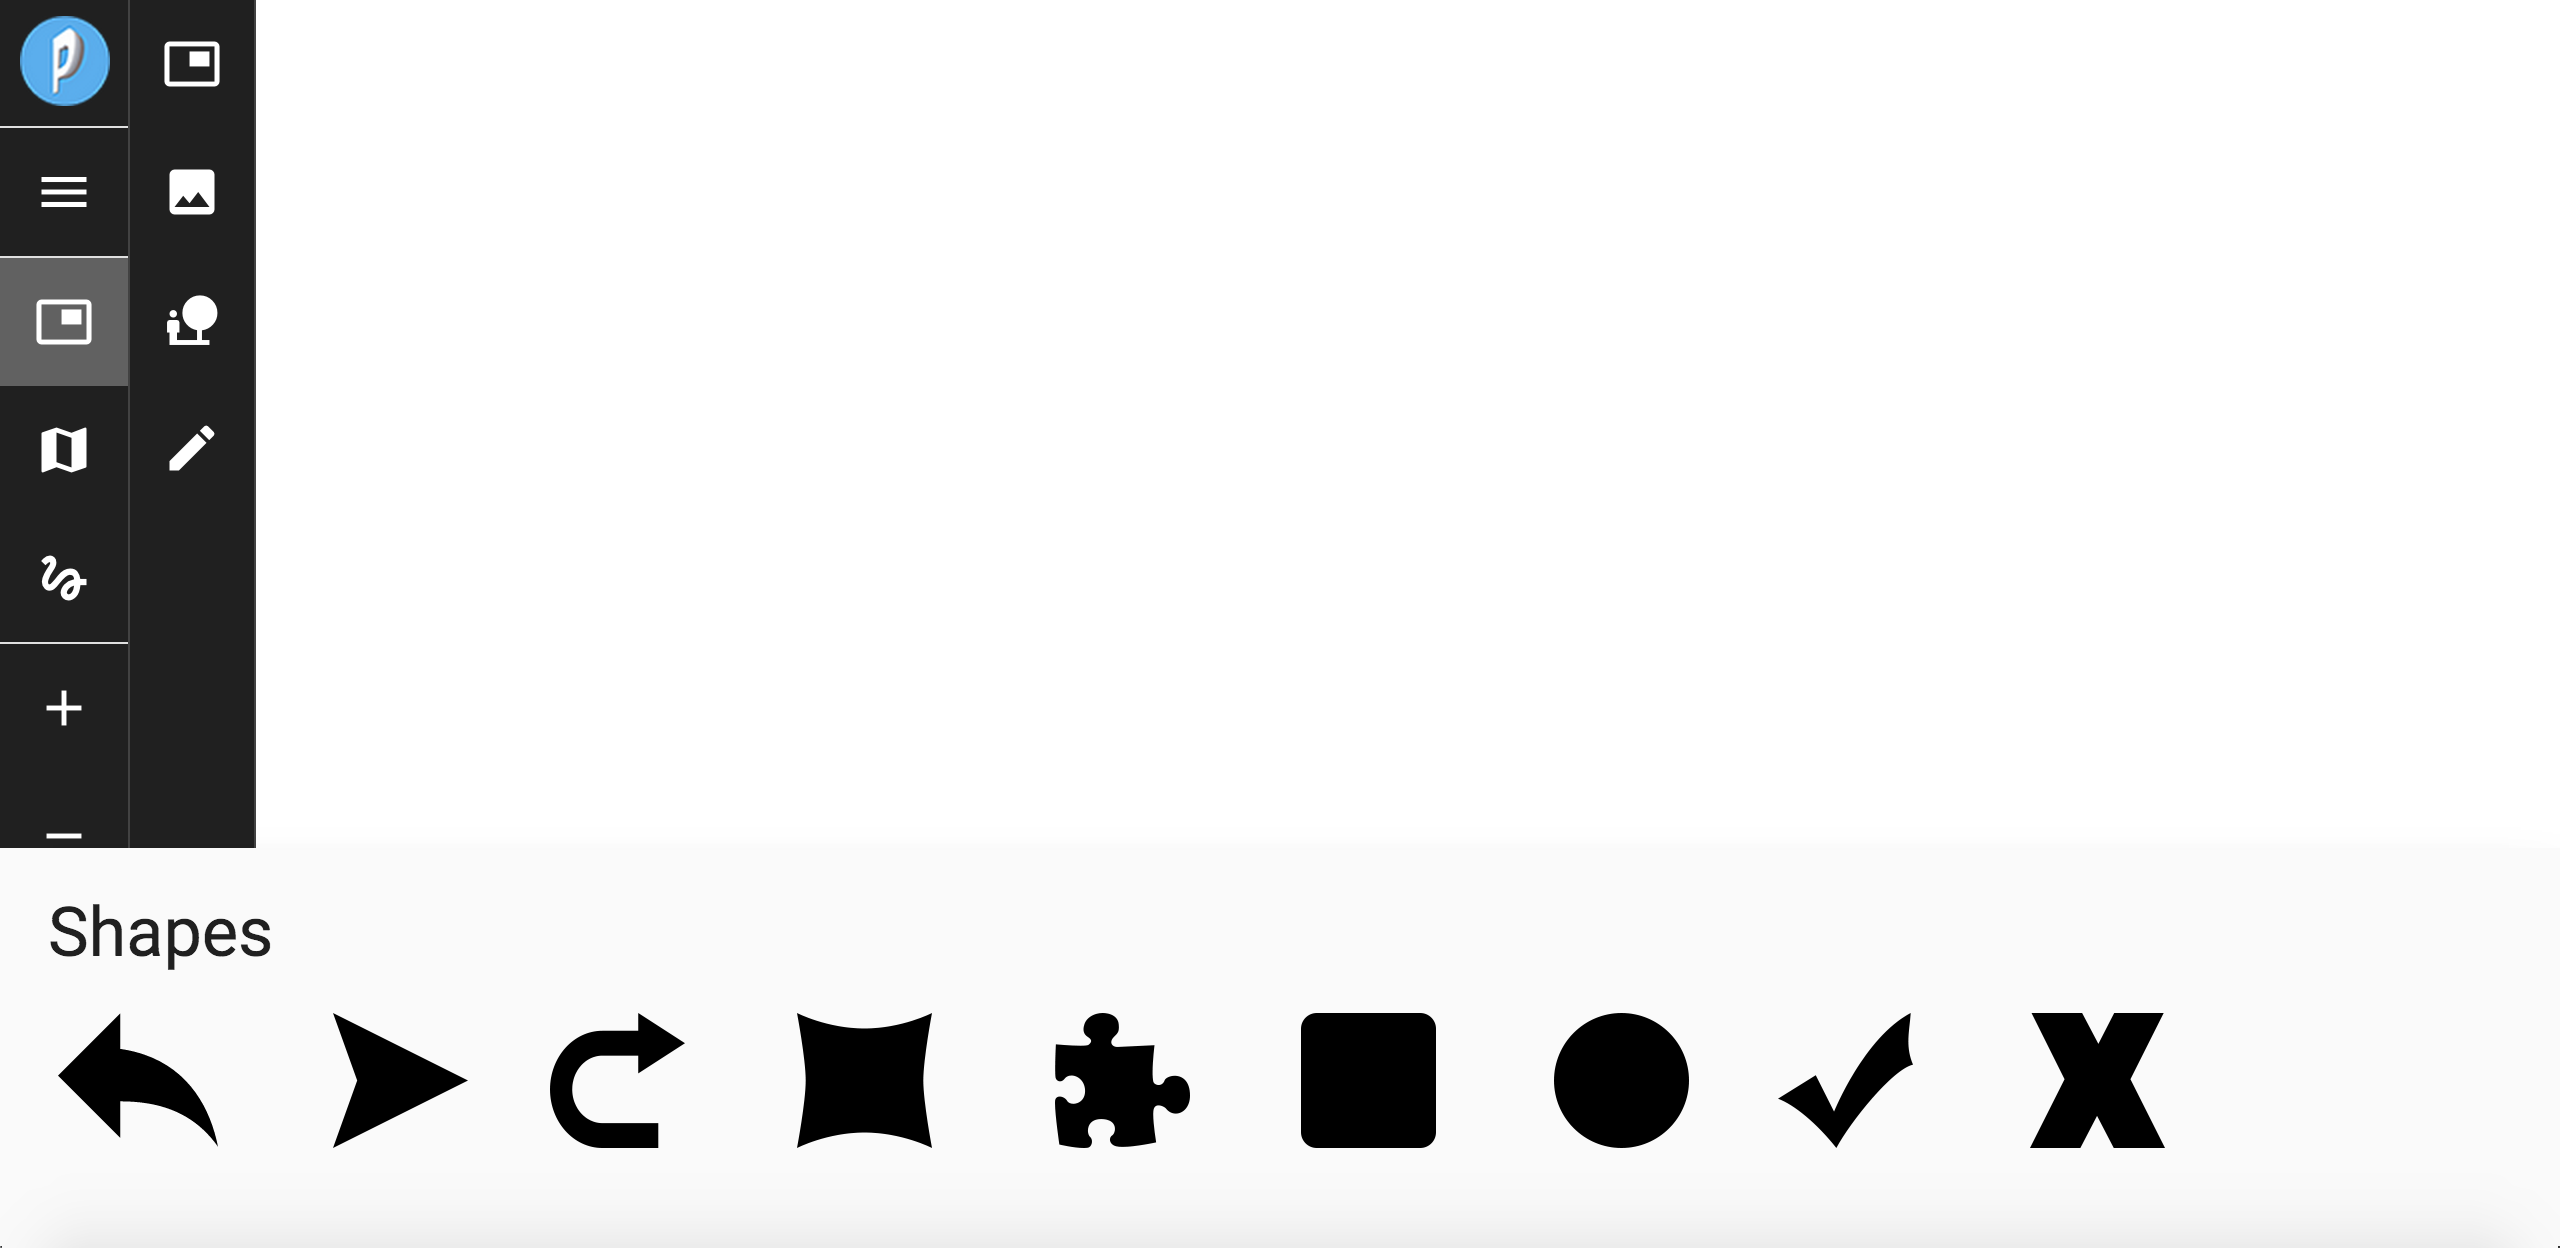
\includegraphics[scale=0.35]{img/sel_shape.png}
\caption{Selezione oggetto forma.}
\end{center}
\end{figure}

Una volta scelta la forma desiderata, questa verrà aggiunta al frame$_G$ corrente.

\subsubsection{Aggiunta testo}
Per aggiungere un'area di testo basterà premere sul comando 
\includegraphics[scale=0.4]{img/add_text.png} visibile nel menu disponibile premendo sul tasto 
\includegraphics[scale=0.4]{img/add_object.png}. \\
Verrà inserita nel frame$_G$ corrente un'area di testo, nella quale sarà possibile inserire il proprio testo.

\subsubsection{Modifica degli elementi}
Per gli oggetti di tipo forma e testo, sarà disponibile un menù che permette la modifica dell'oggetto selezionato.\\
Per accedere a questo menù sarà sufficiente selezionare l'oggetto con un click.\\
Questo menù varia a seconda del tipo di oggetto selezionato.\\
Per un oggetto di tipo testo è possibile modificarne la formattazione:
\begin{figure}[!h]
\begin{center}
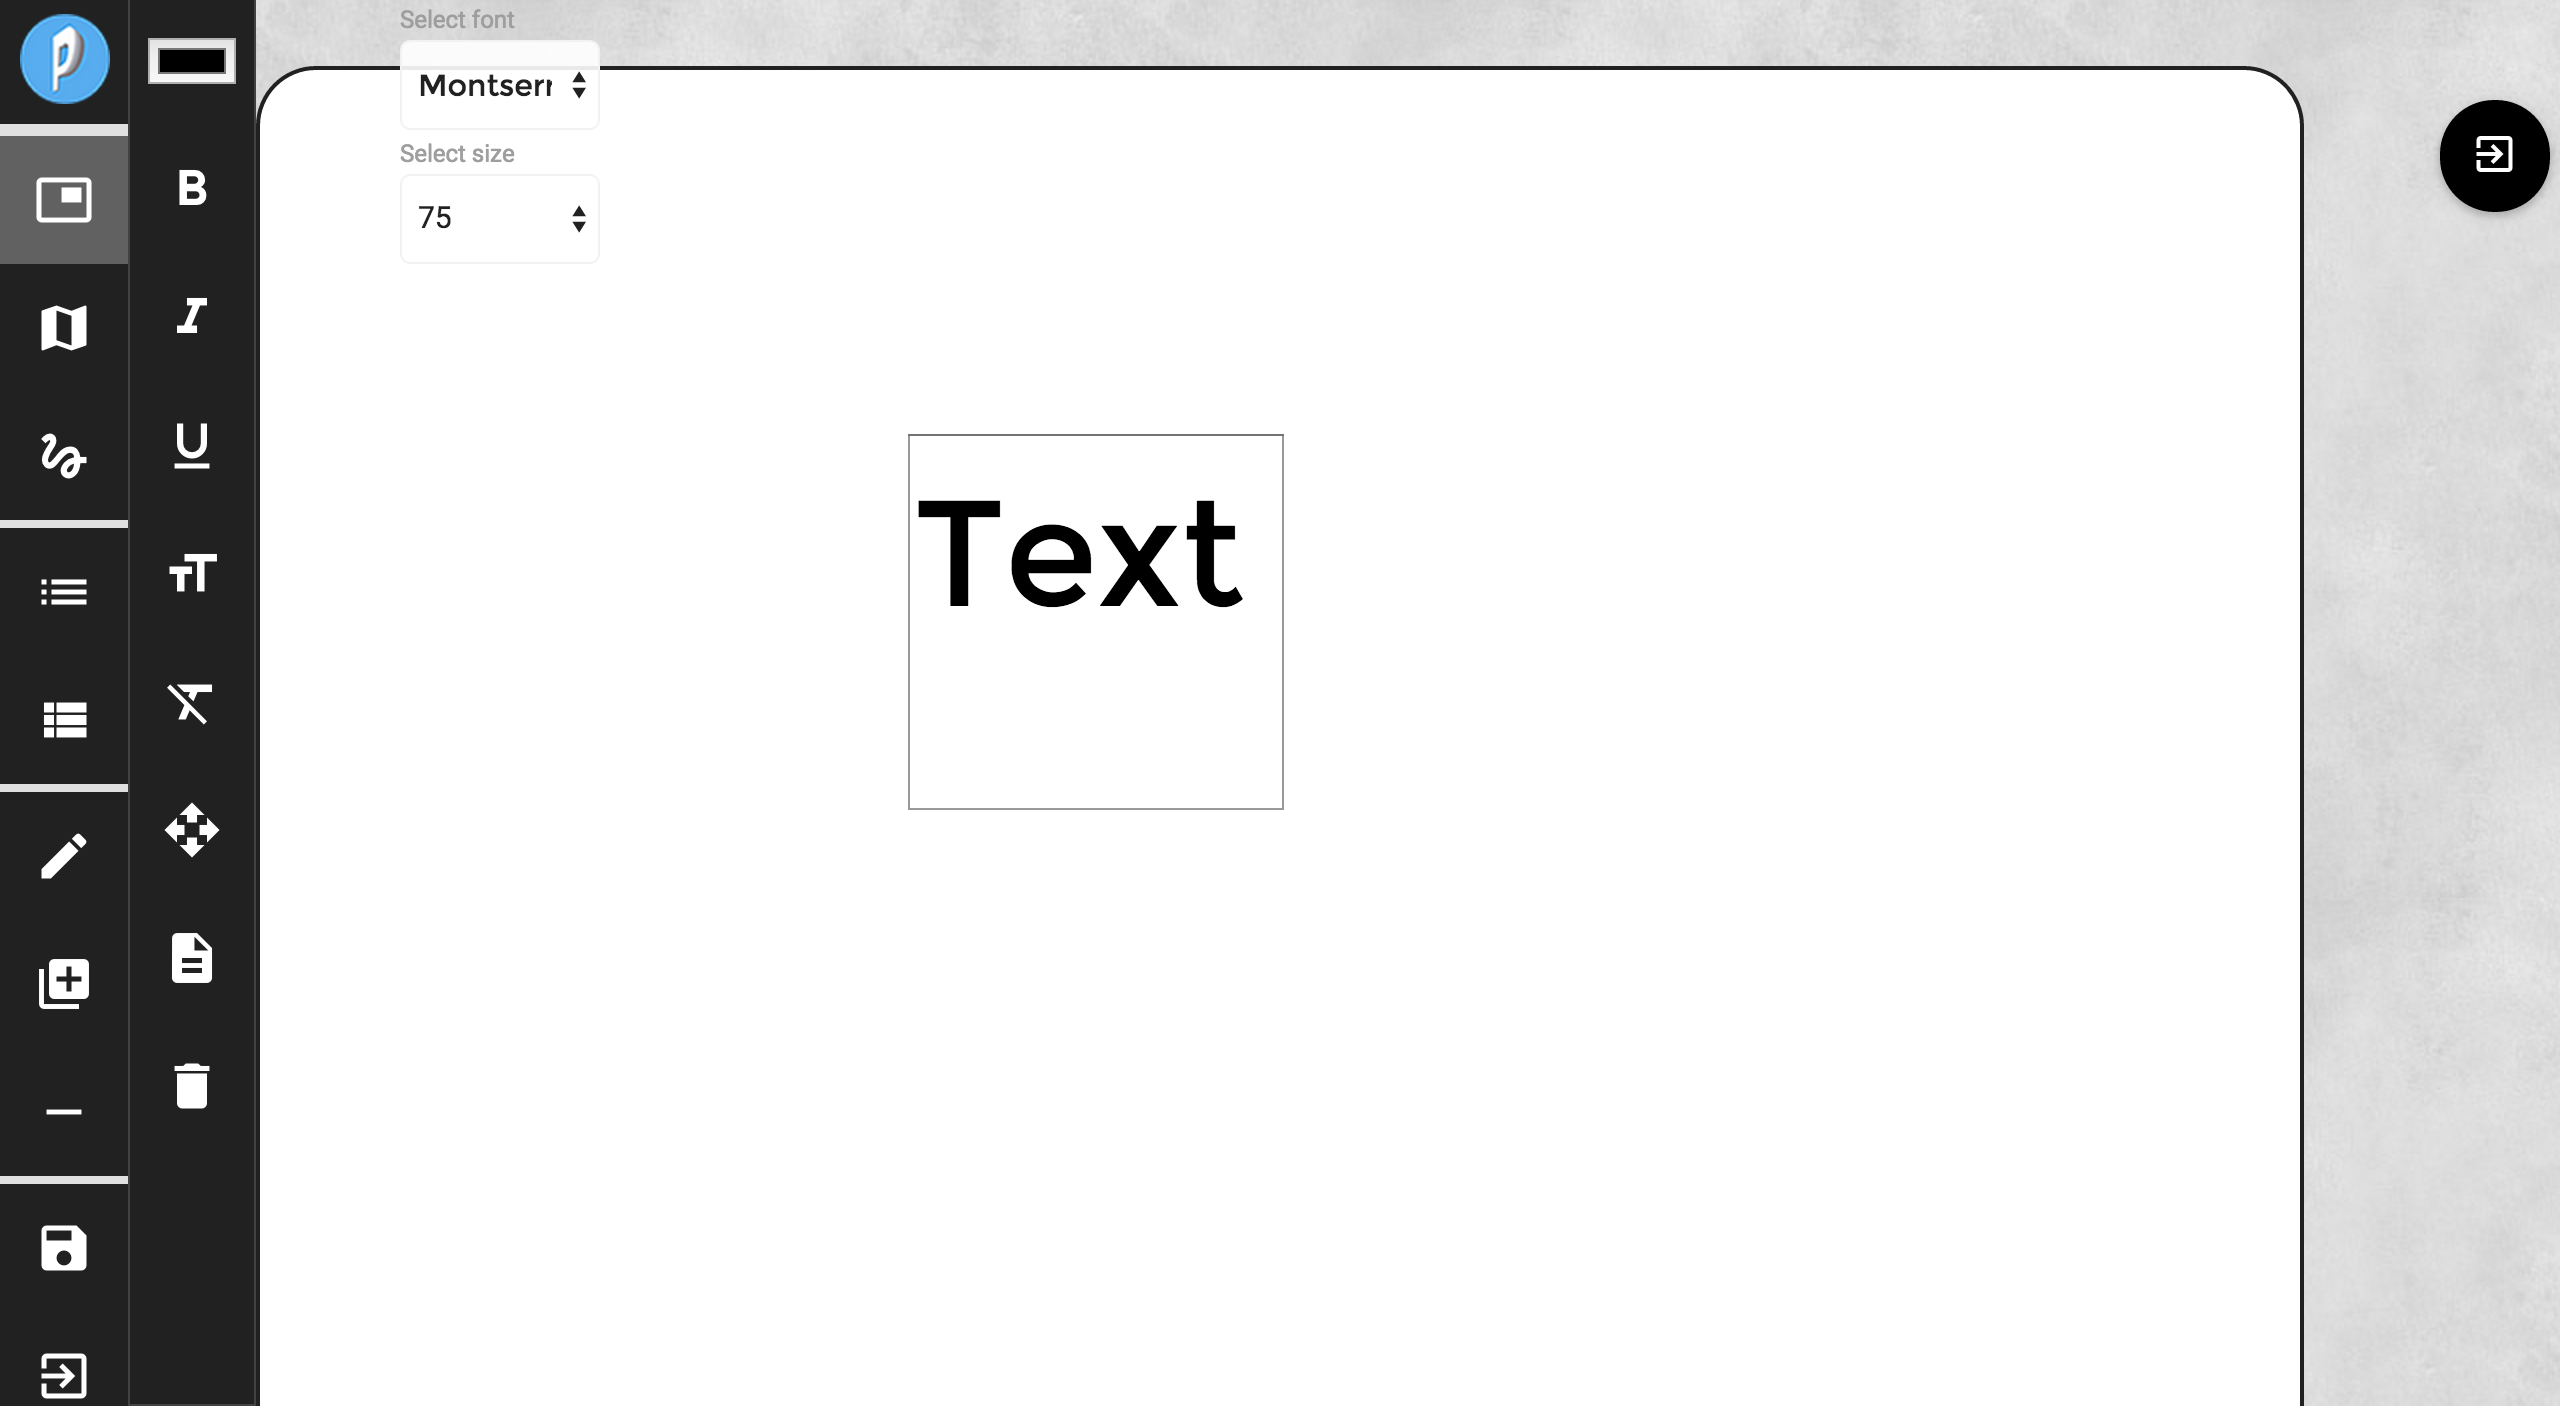
\includegraphics[scale=0.35]{img/edit_text.png}
\caption{Modifica testo.}
\end{center}
\end{figure}
\newpage
Per un oggetto di tipo forma è possibile modificare il suo colore o il tipo della forma.\\
\begin{figure}[!h]
\begin{center}
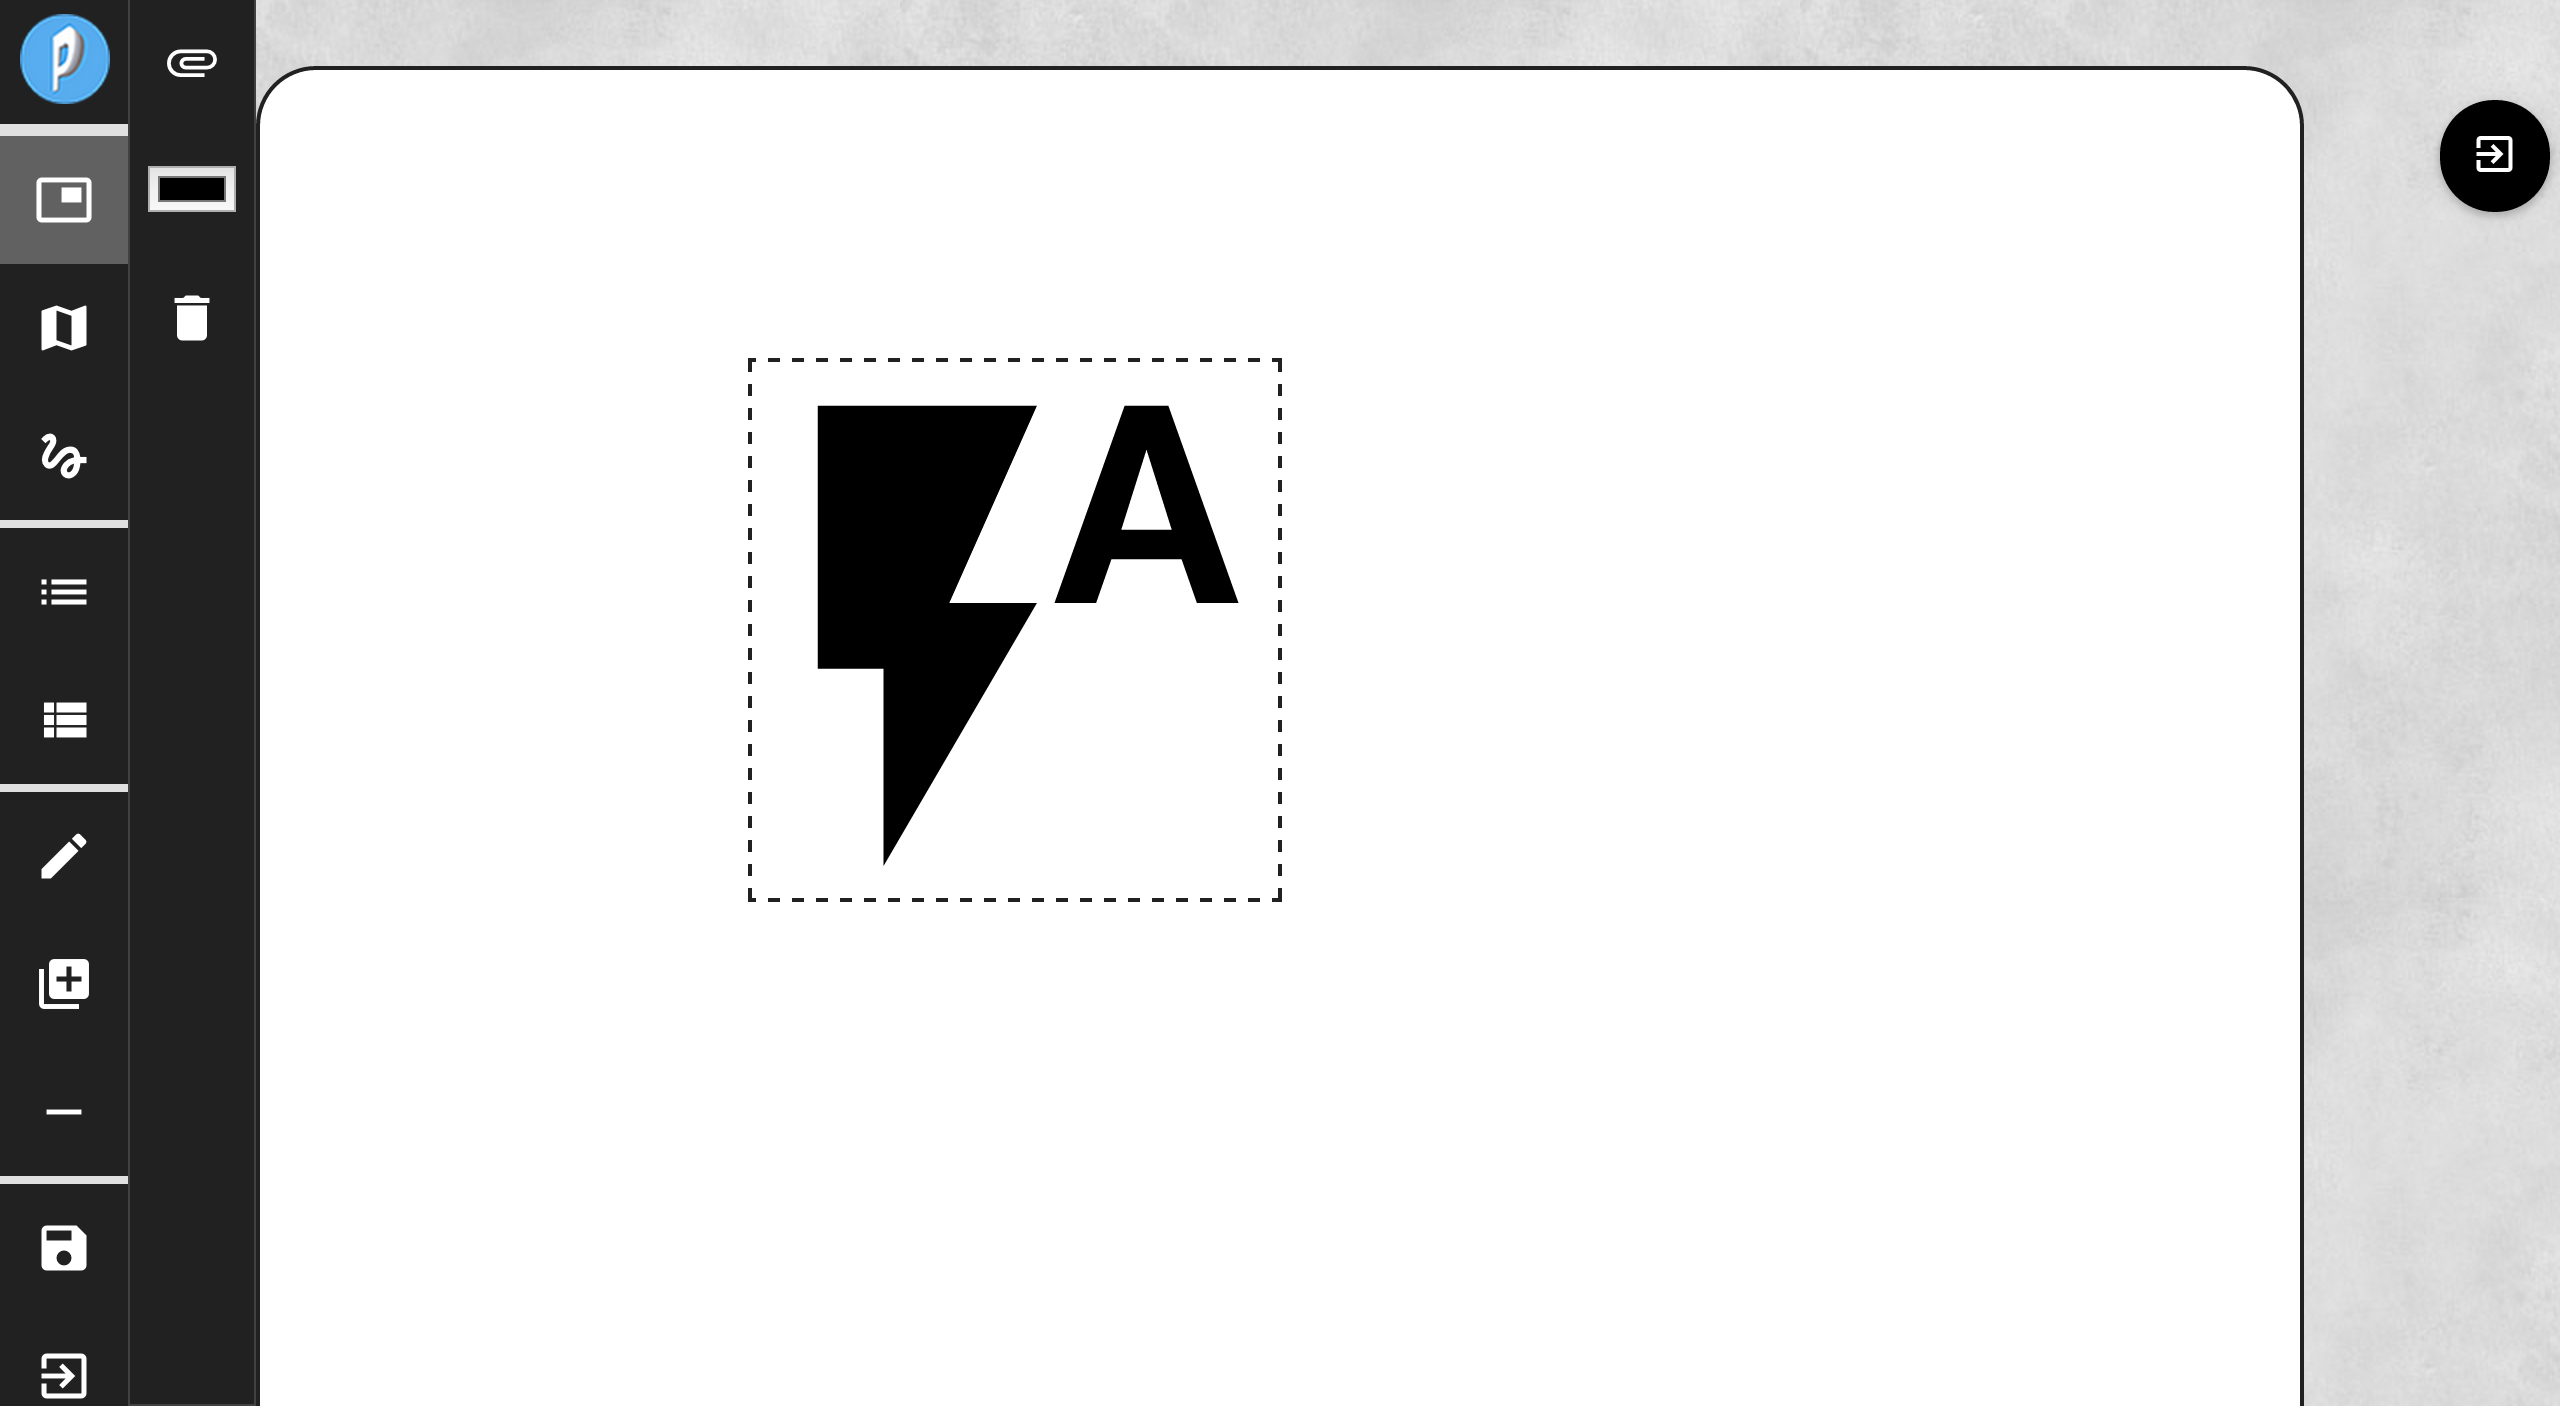
\includegraphics[scale=0.35]{img/edit_shape.png}
\caption{Modifica forma.}
\end{center}
\end{figure}

\newpage
\subsection{Infographic editor$_G$}
Questa modalità permette di modificare l'infografica$_G$ risultante dalla presentazione finora creata.
\begin{figure}[!h]
\begin{center}
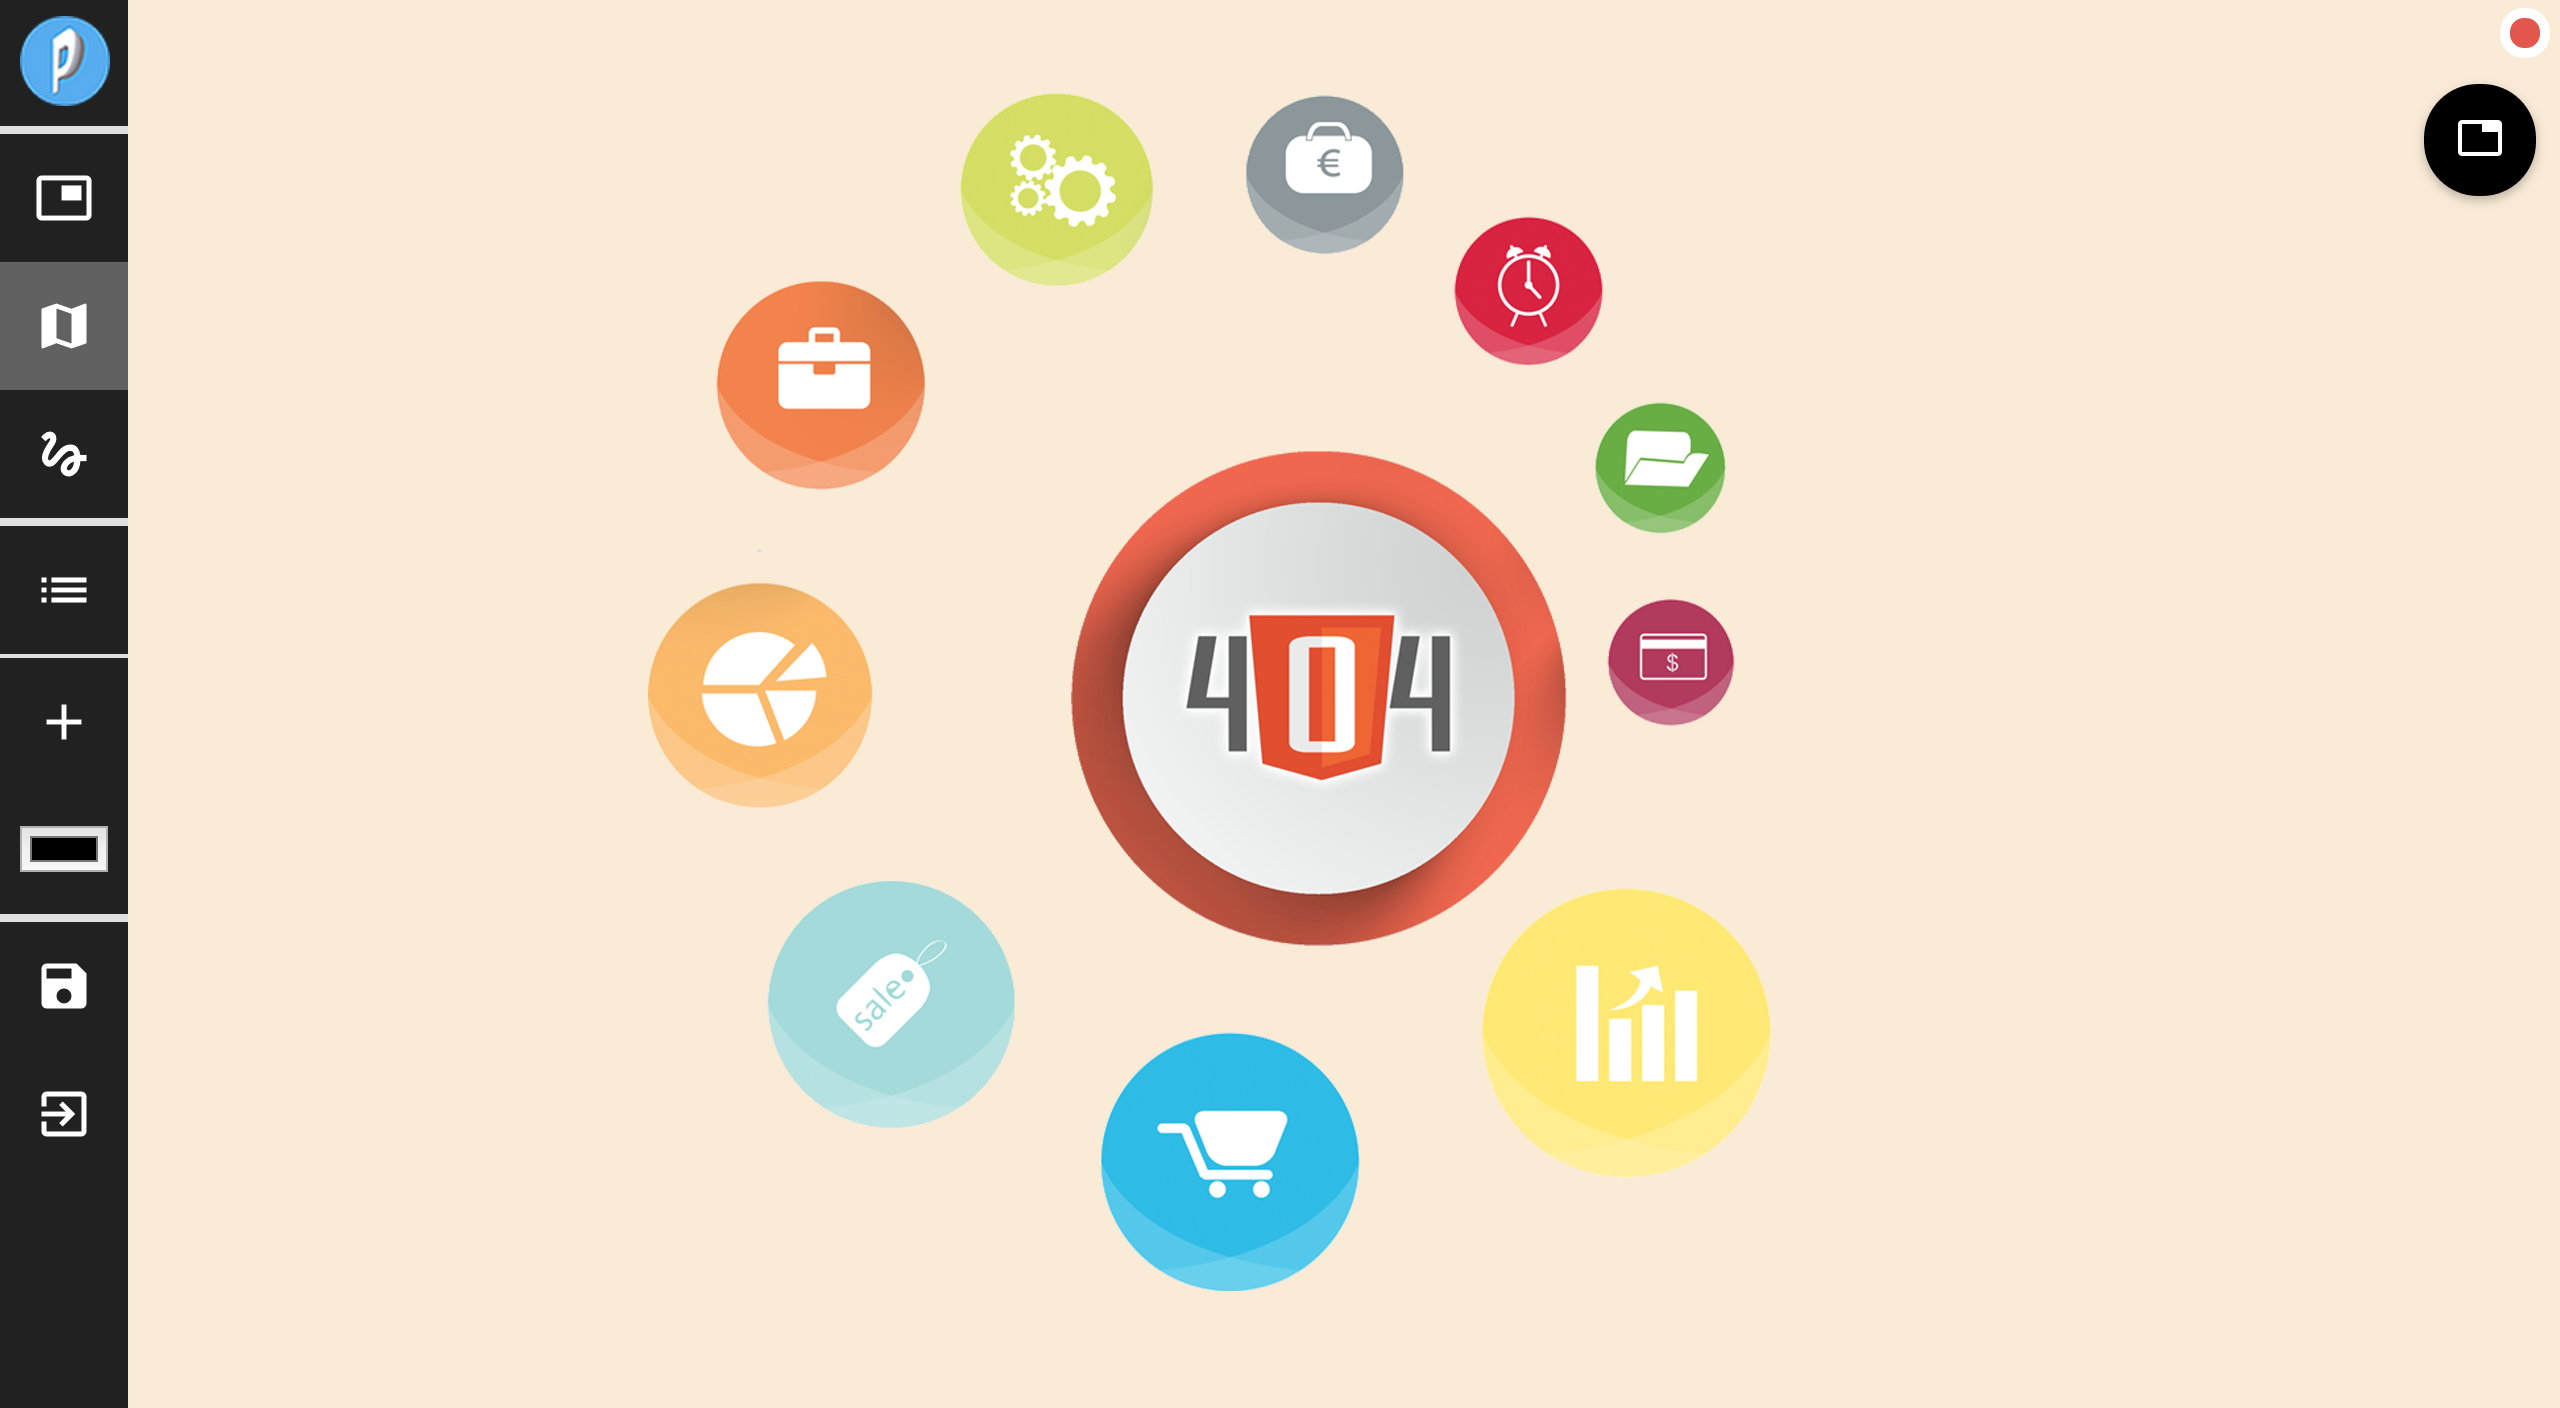
\includegraphics[scale=0.35]{img/infographic.png}
\caption{Infographic editor$_G$.}
\end{center}
\end{figure}

Anche in questa modalità è possibile aggiungere un oggetto (testo, immagine o forma) all'infografica$_G$ tramite il comando 
\includegraphics[scale=0.4]{img/add_object.png}.\\
La lista dei frame$_G$ già presenti all'interno dell'infografica$_G$ è visualizzabile premendo il pulsante 
\includegraphics[scale=0.4]{img/added_frames.png}.
Mentre per visualizzare i frame$_G$s che non sono ancora stati aggiunti all'infografica$_G$ sarà sufficiente premere sul pulsante 
\includegraphics[scale=0.4]{img/frames_to_be_added.png}.\\
Una volta aggiunti i frames$_G$ sarà possibile spostarli all'interno dell'infografica$_G$ semplicemente trascinandoli col mouse.

\subsection{Trails editor$_G$}
Con la modalità \emph{Trails editor$_G$} è possibile gestire i cammini presentativi, ovvero, per una stessa presentazione, è possibile impostare diversi modi in cui scorrere i frames$_G$. Sarà possibile selezionare uno dei cammini prima dell'avvio della presentazione.\\

\begin{figure}[!h]
\begin{center}
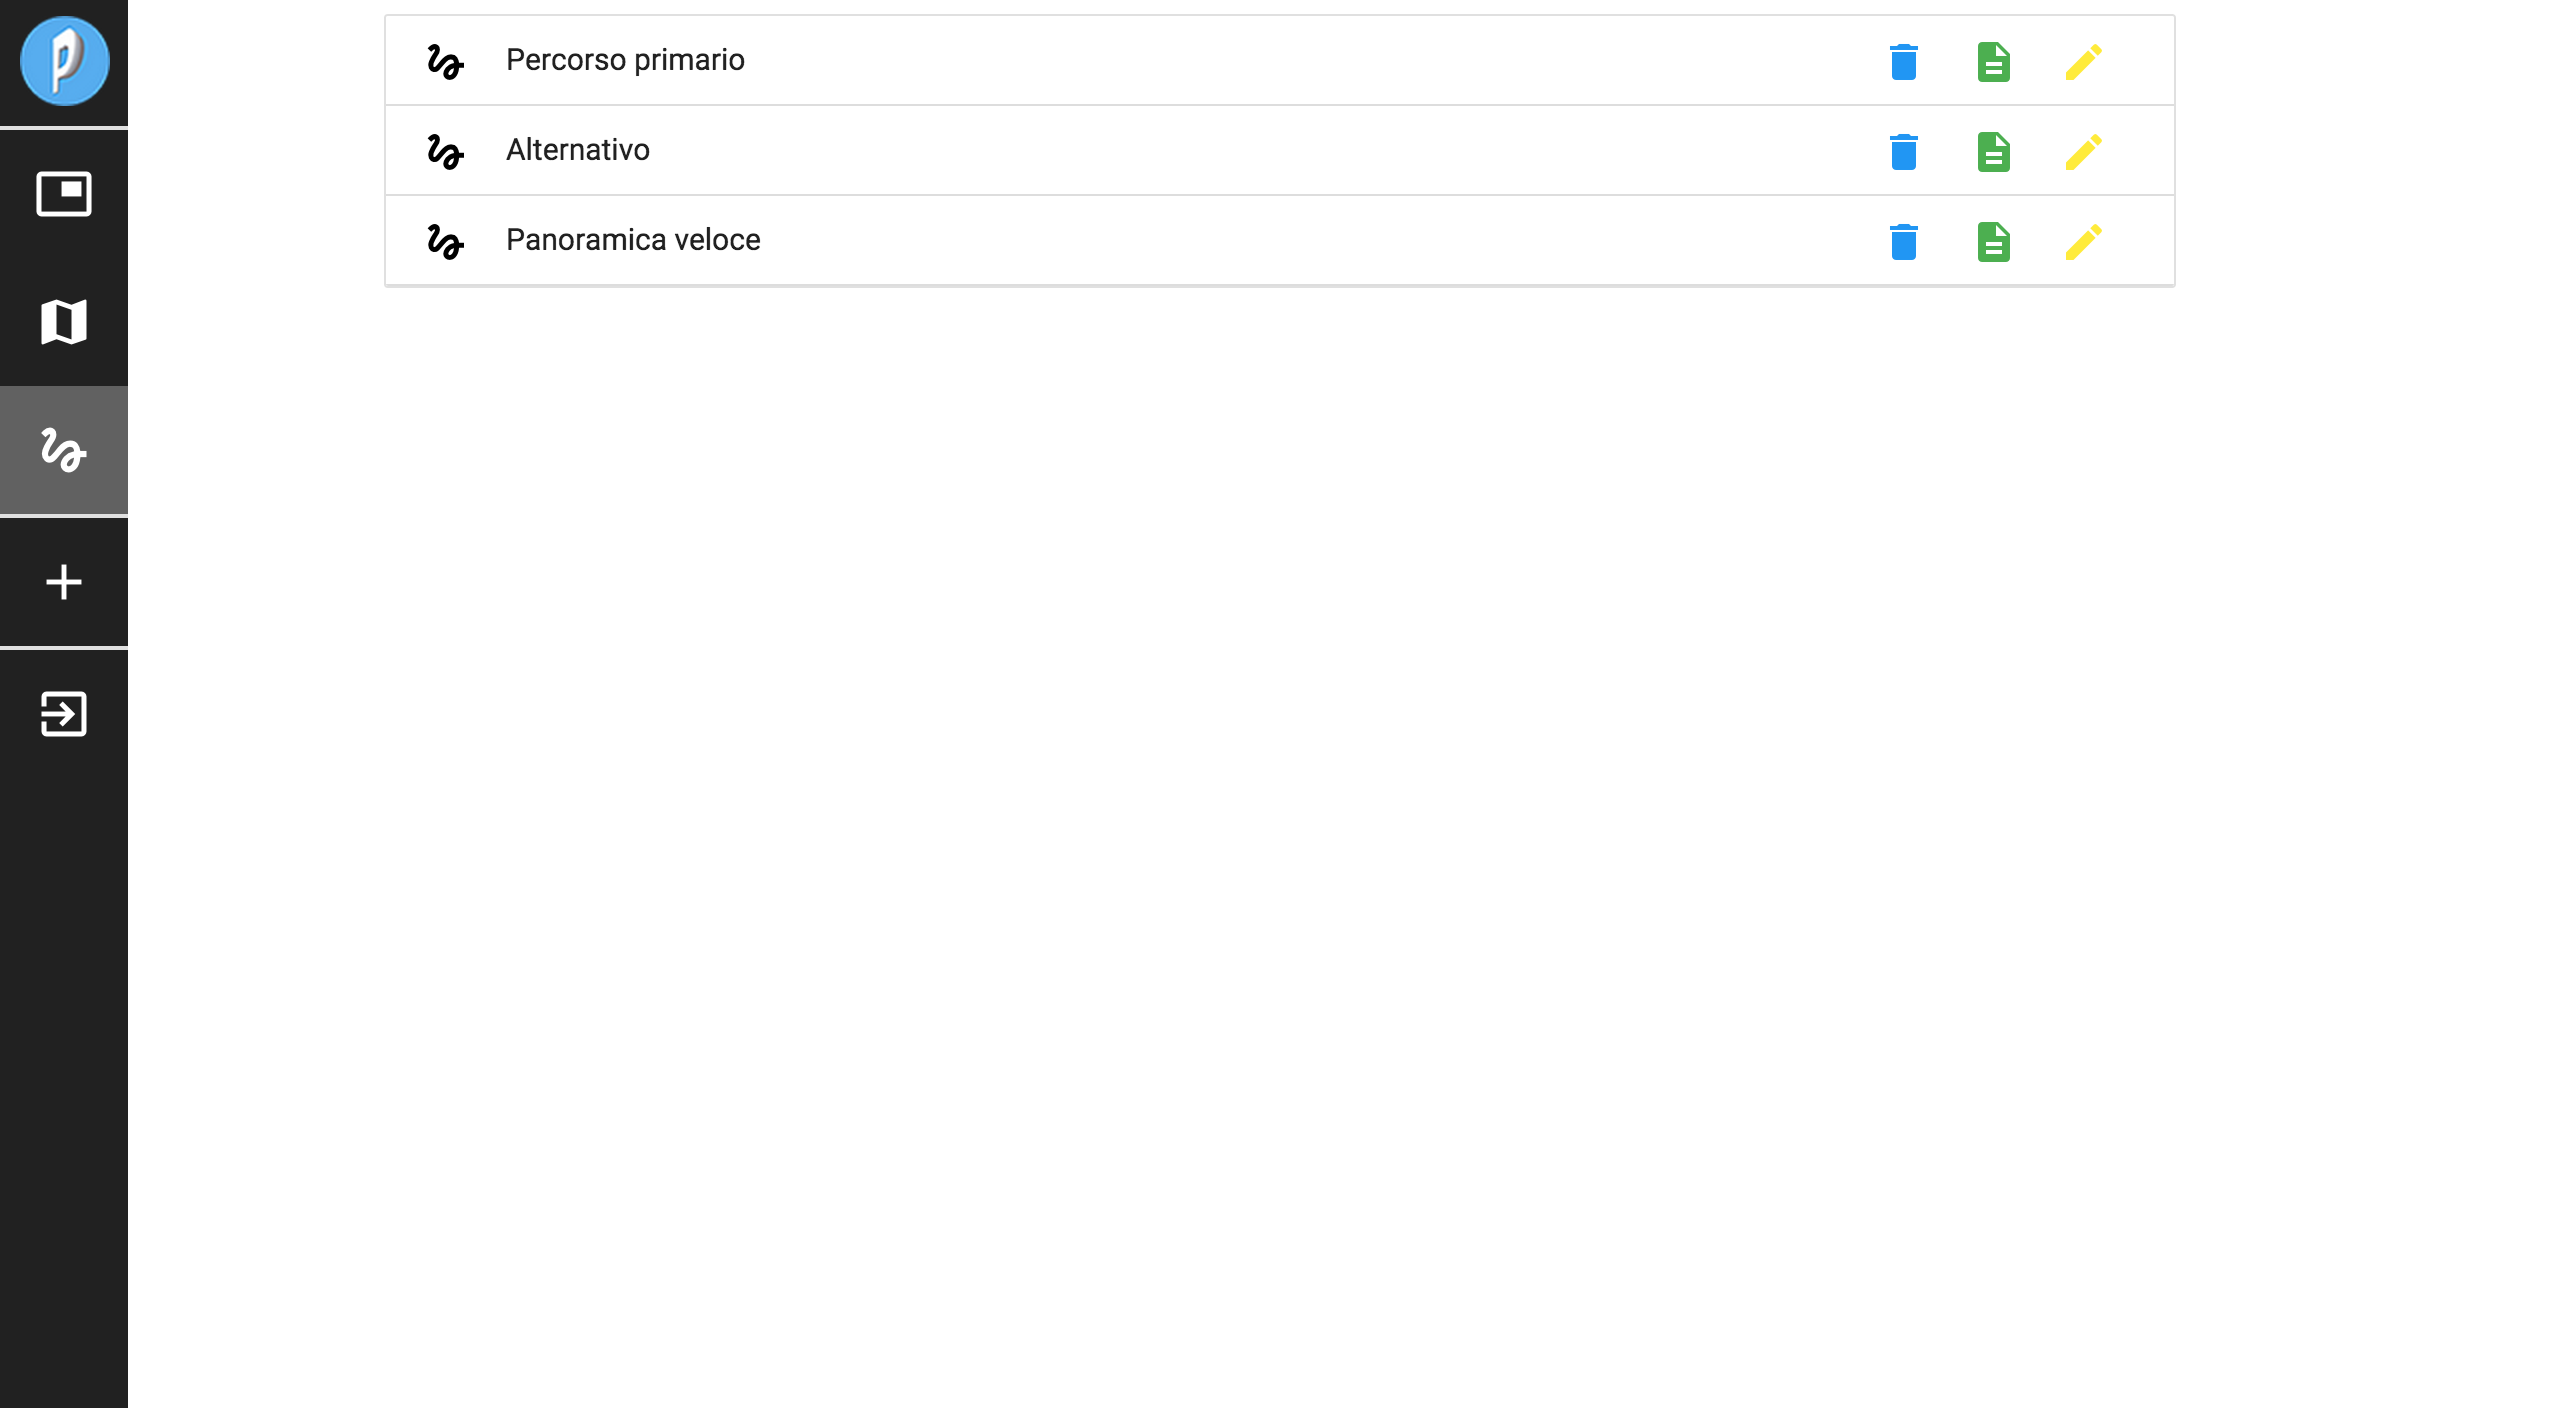
\includegraphics[scale=0.35]{img/trails_editor_screen.png}
\caption{Modalità Trails editor$_G$.}
\end{center}
\end{figure}

Per creare un nuovo cammino premere sul comando 
\includegraphics[scale=0.4]{img/add_object.png}. Verrà chiesto di inserire un titolo per il nuovo cammino. Premere quindi su 
\includegraphics[scale=0.5]{img/save_confirm.png}.\\
Il nuovo cammino appena creato verrà aggiunto alla lista dei cammini presenti.\\
Per modificare la struttura di un cammino selezionare l'icona 
\includegraphics[scale=0.7]{img/edit.png} corrispondente al cammino che si vuole modificare.

\subsubsection{Creazione percorso presentativo}
Una volta selezionato il percorso da modificare sarà possibile aggiungere i vari frames$_G$ e gestirne l'ordine di visualizzazione.

\begin{figure}[!h]
\begin{center}
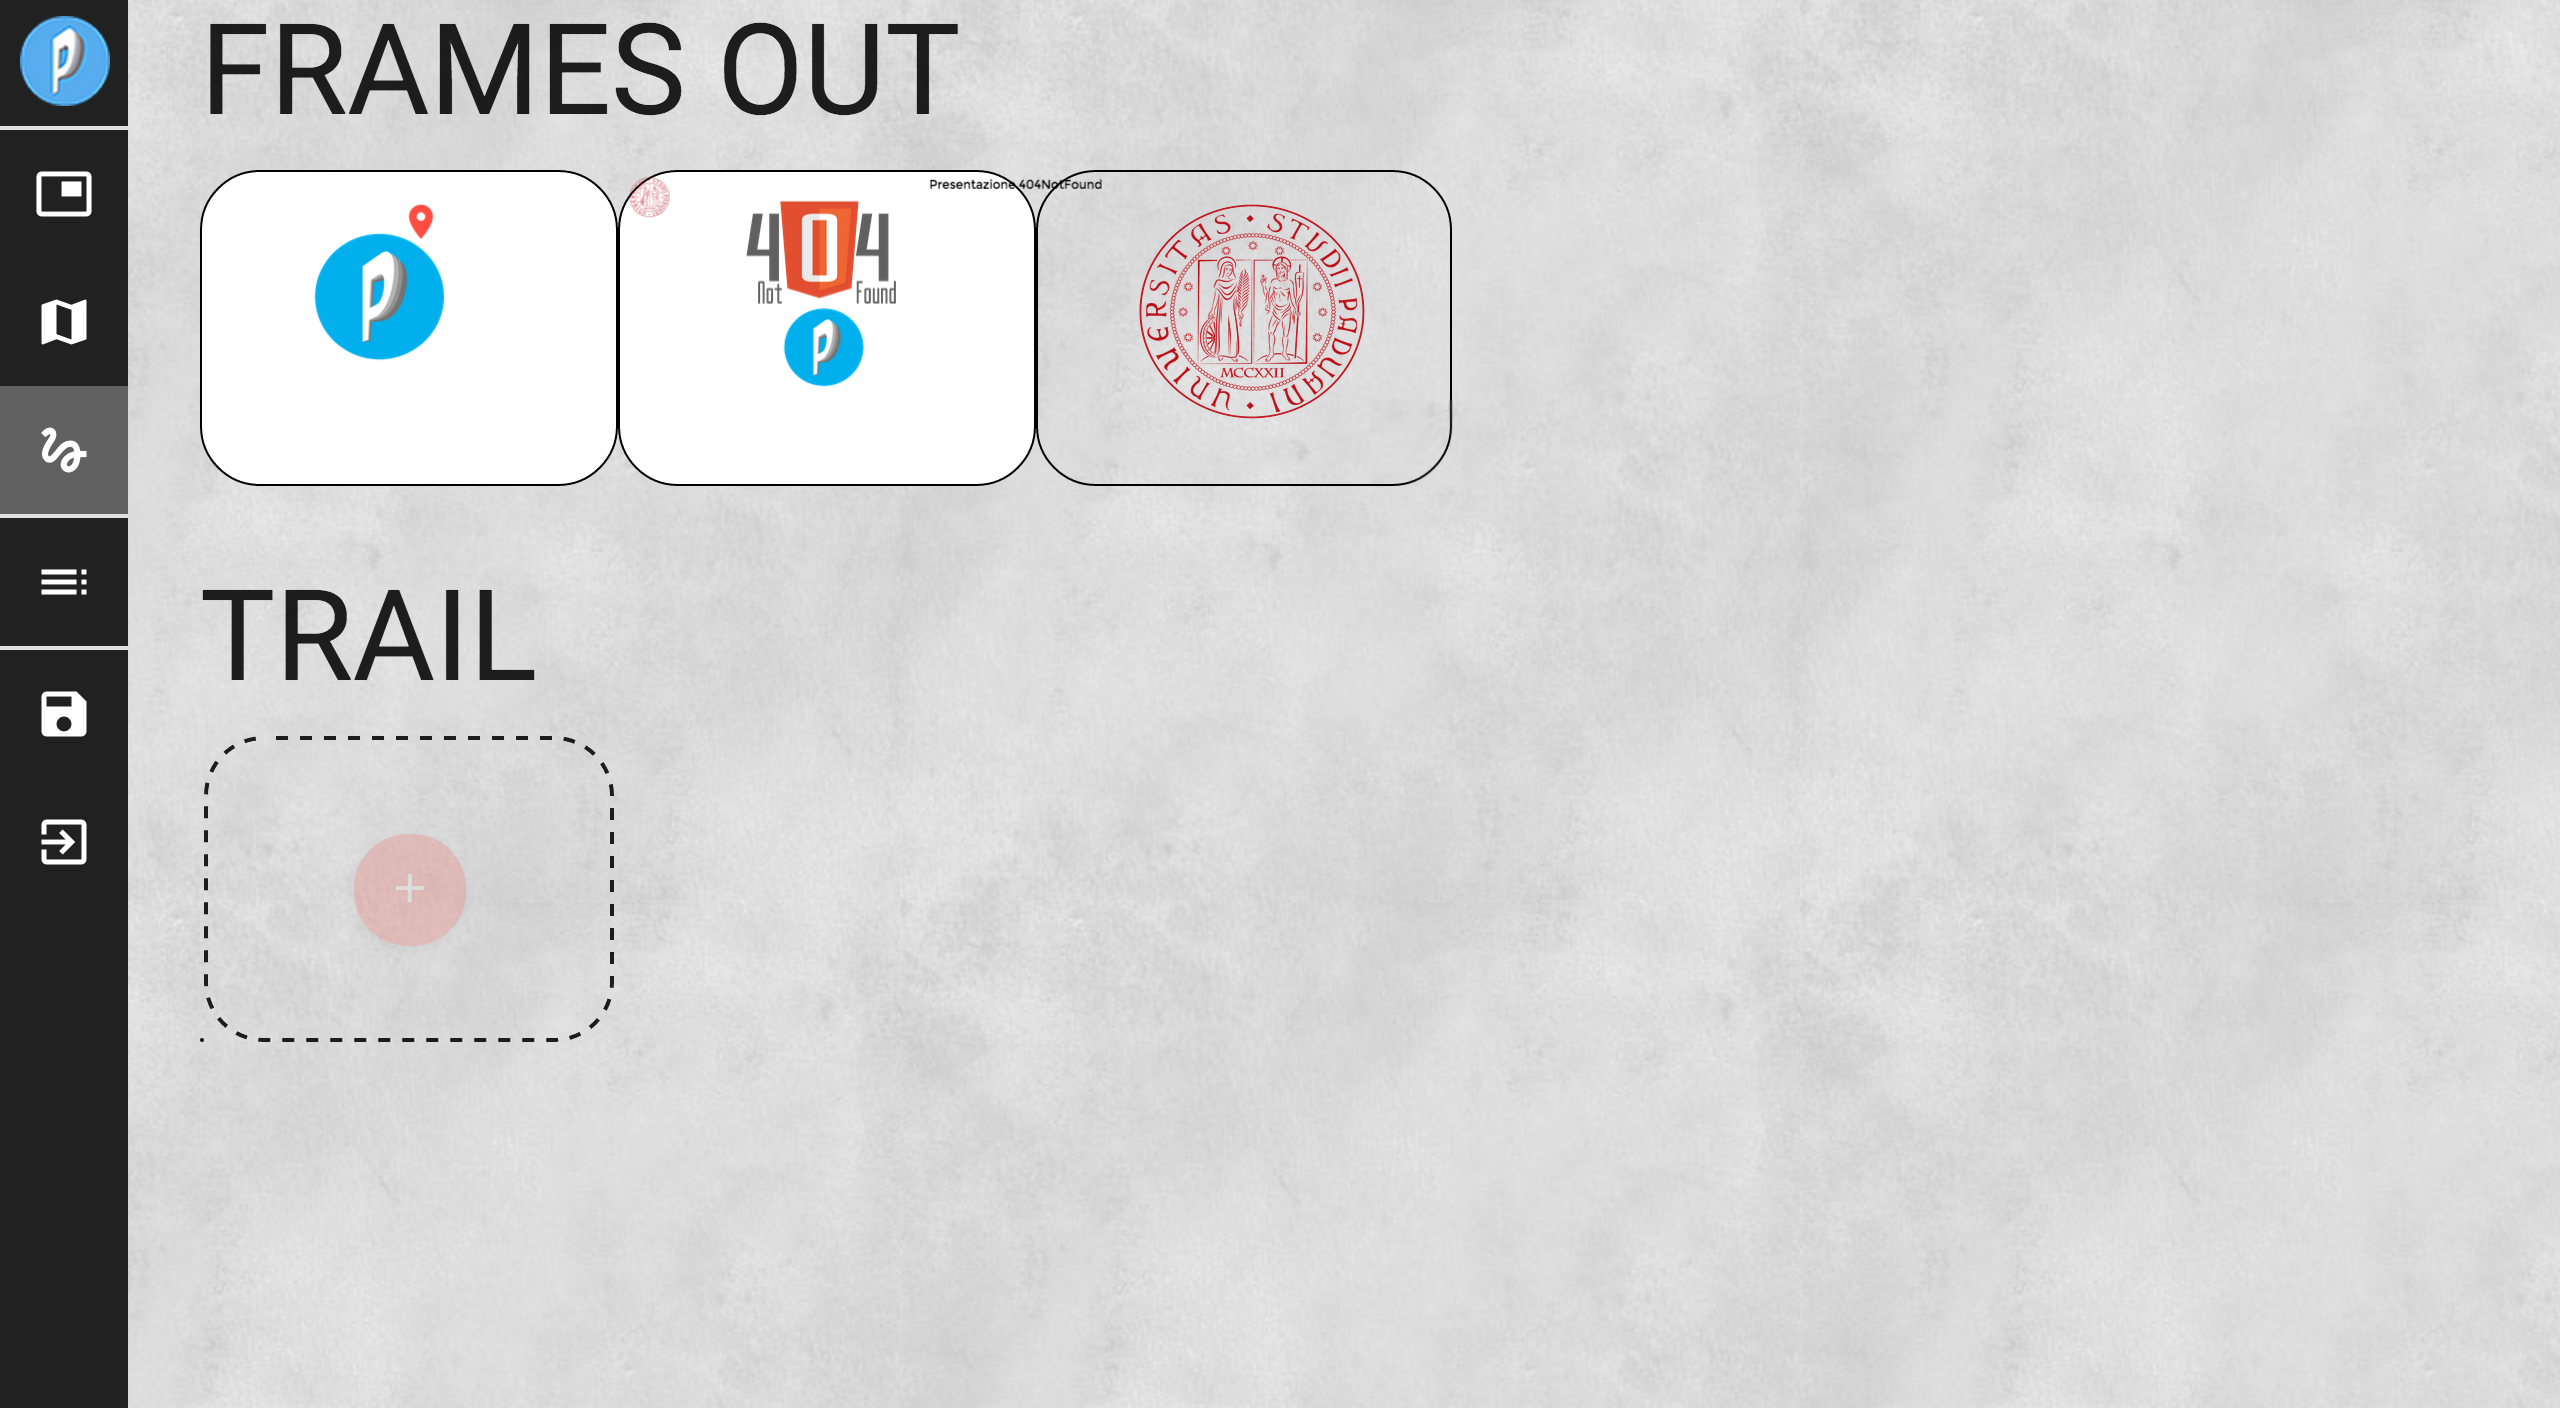
\includegraphics[scale=0.35]{img/edit_trail.png}
\caption{Modalità Trails editor$_G$.}
\end{center}
\end{figure}

Per aggiungere un frame$_G$ al percorso si deve prima selezionare dalla lista dei frames $_G$, visualizzabile premendo sul pulsante 
\includegraphics[scale=0.4]{img/frames_to_be_added.png} e successivamente premendo sul pulsante 
\includegraphics[scale=0.4]{img/add.png} corrispondente alla direzione in cui si vuole inserire il frame$_G$.\\

\begin{figure}[!h]
\begin{center}
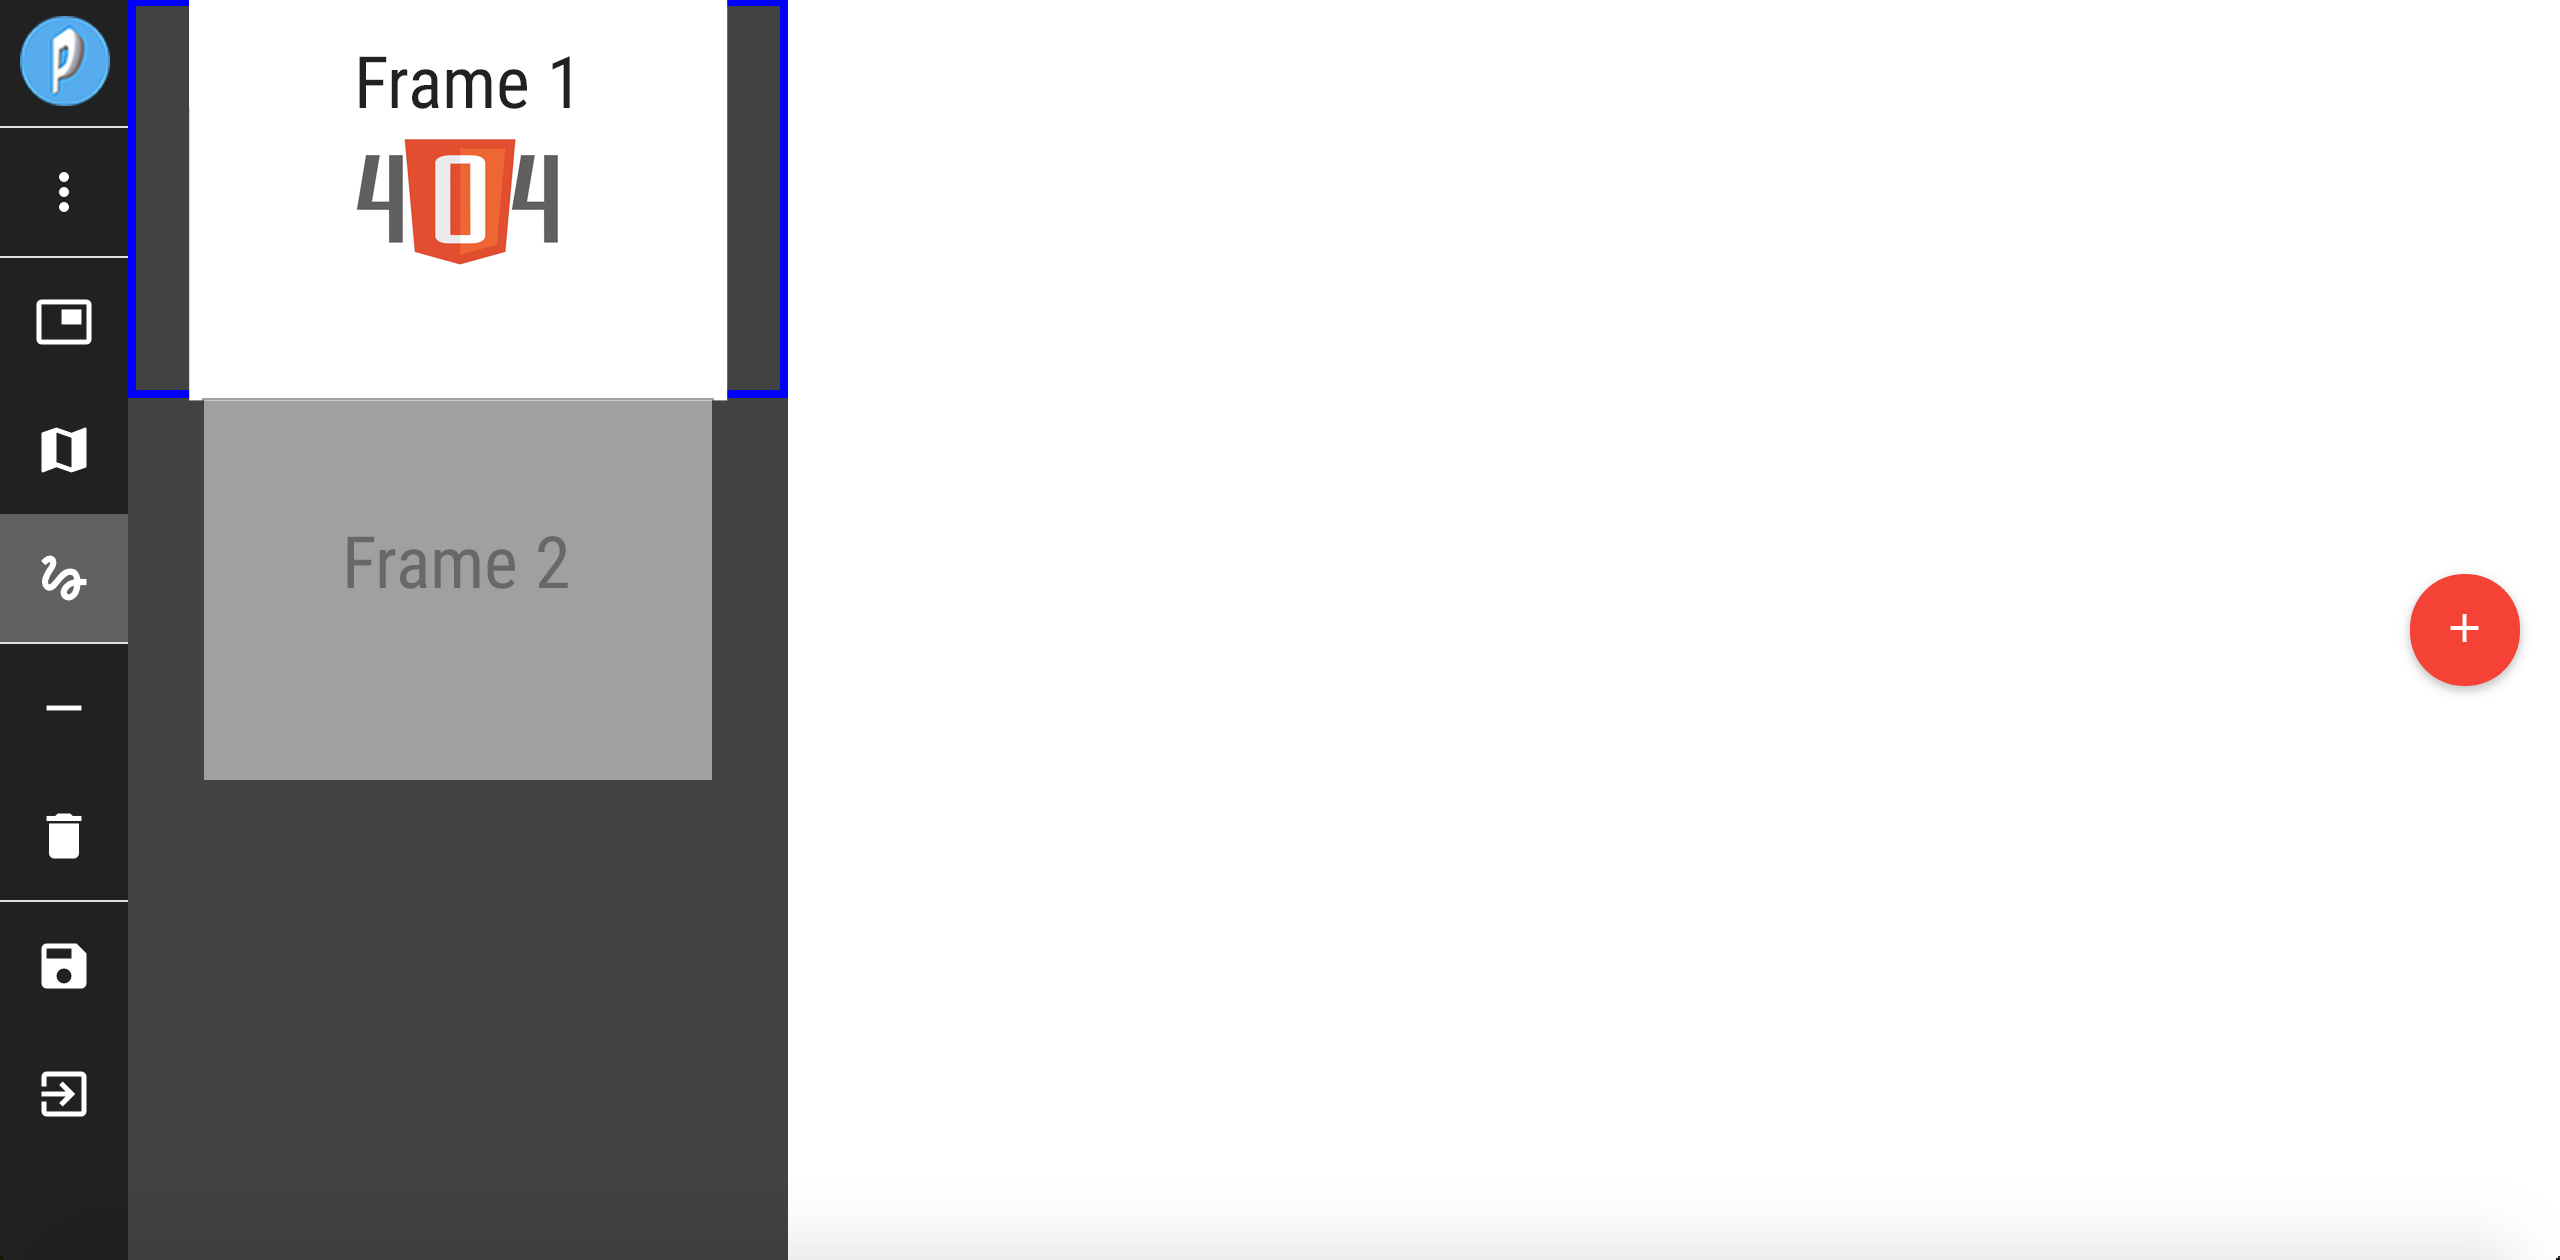
\includegraphics[scale=0.35]{img/trail_frames_list.png}
\caption{Modalità Trails editor$_G$.}
\end{center}
\end{figure}

Una volta inserito il frame$_G$ sarà possibile ripetere la procedura per inserire un ulteriore frame$_G$ oppure marcare quello corrente come checkpoint$_G$, ovvero impostarlo come nodo di partenza di un percorso alternativo, premendo sul pulsante 
\includegraphics[scale=0.4]{img/checkpoint.png}.\\

\begin{figure}[!h]
\begin{center}
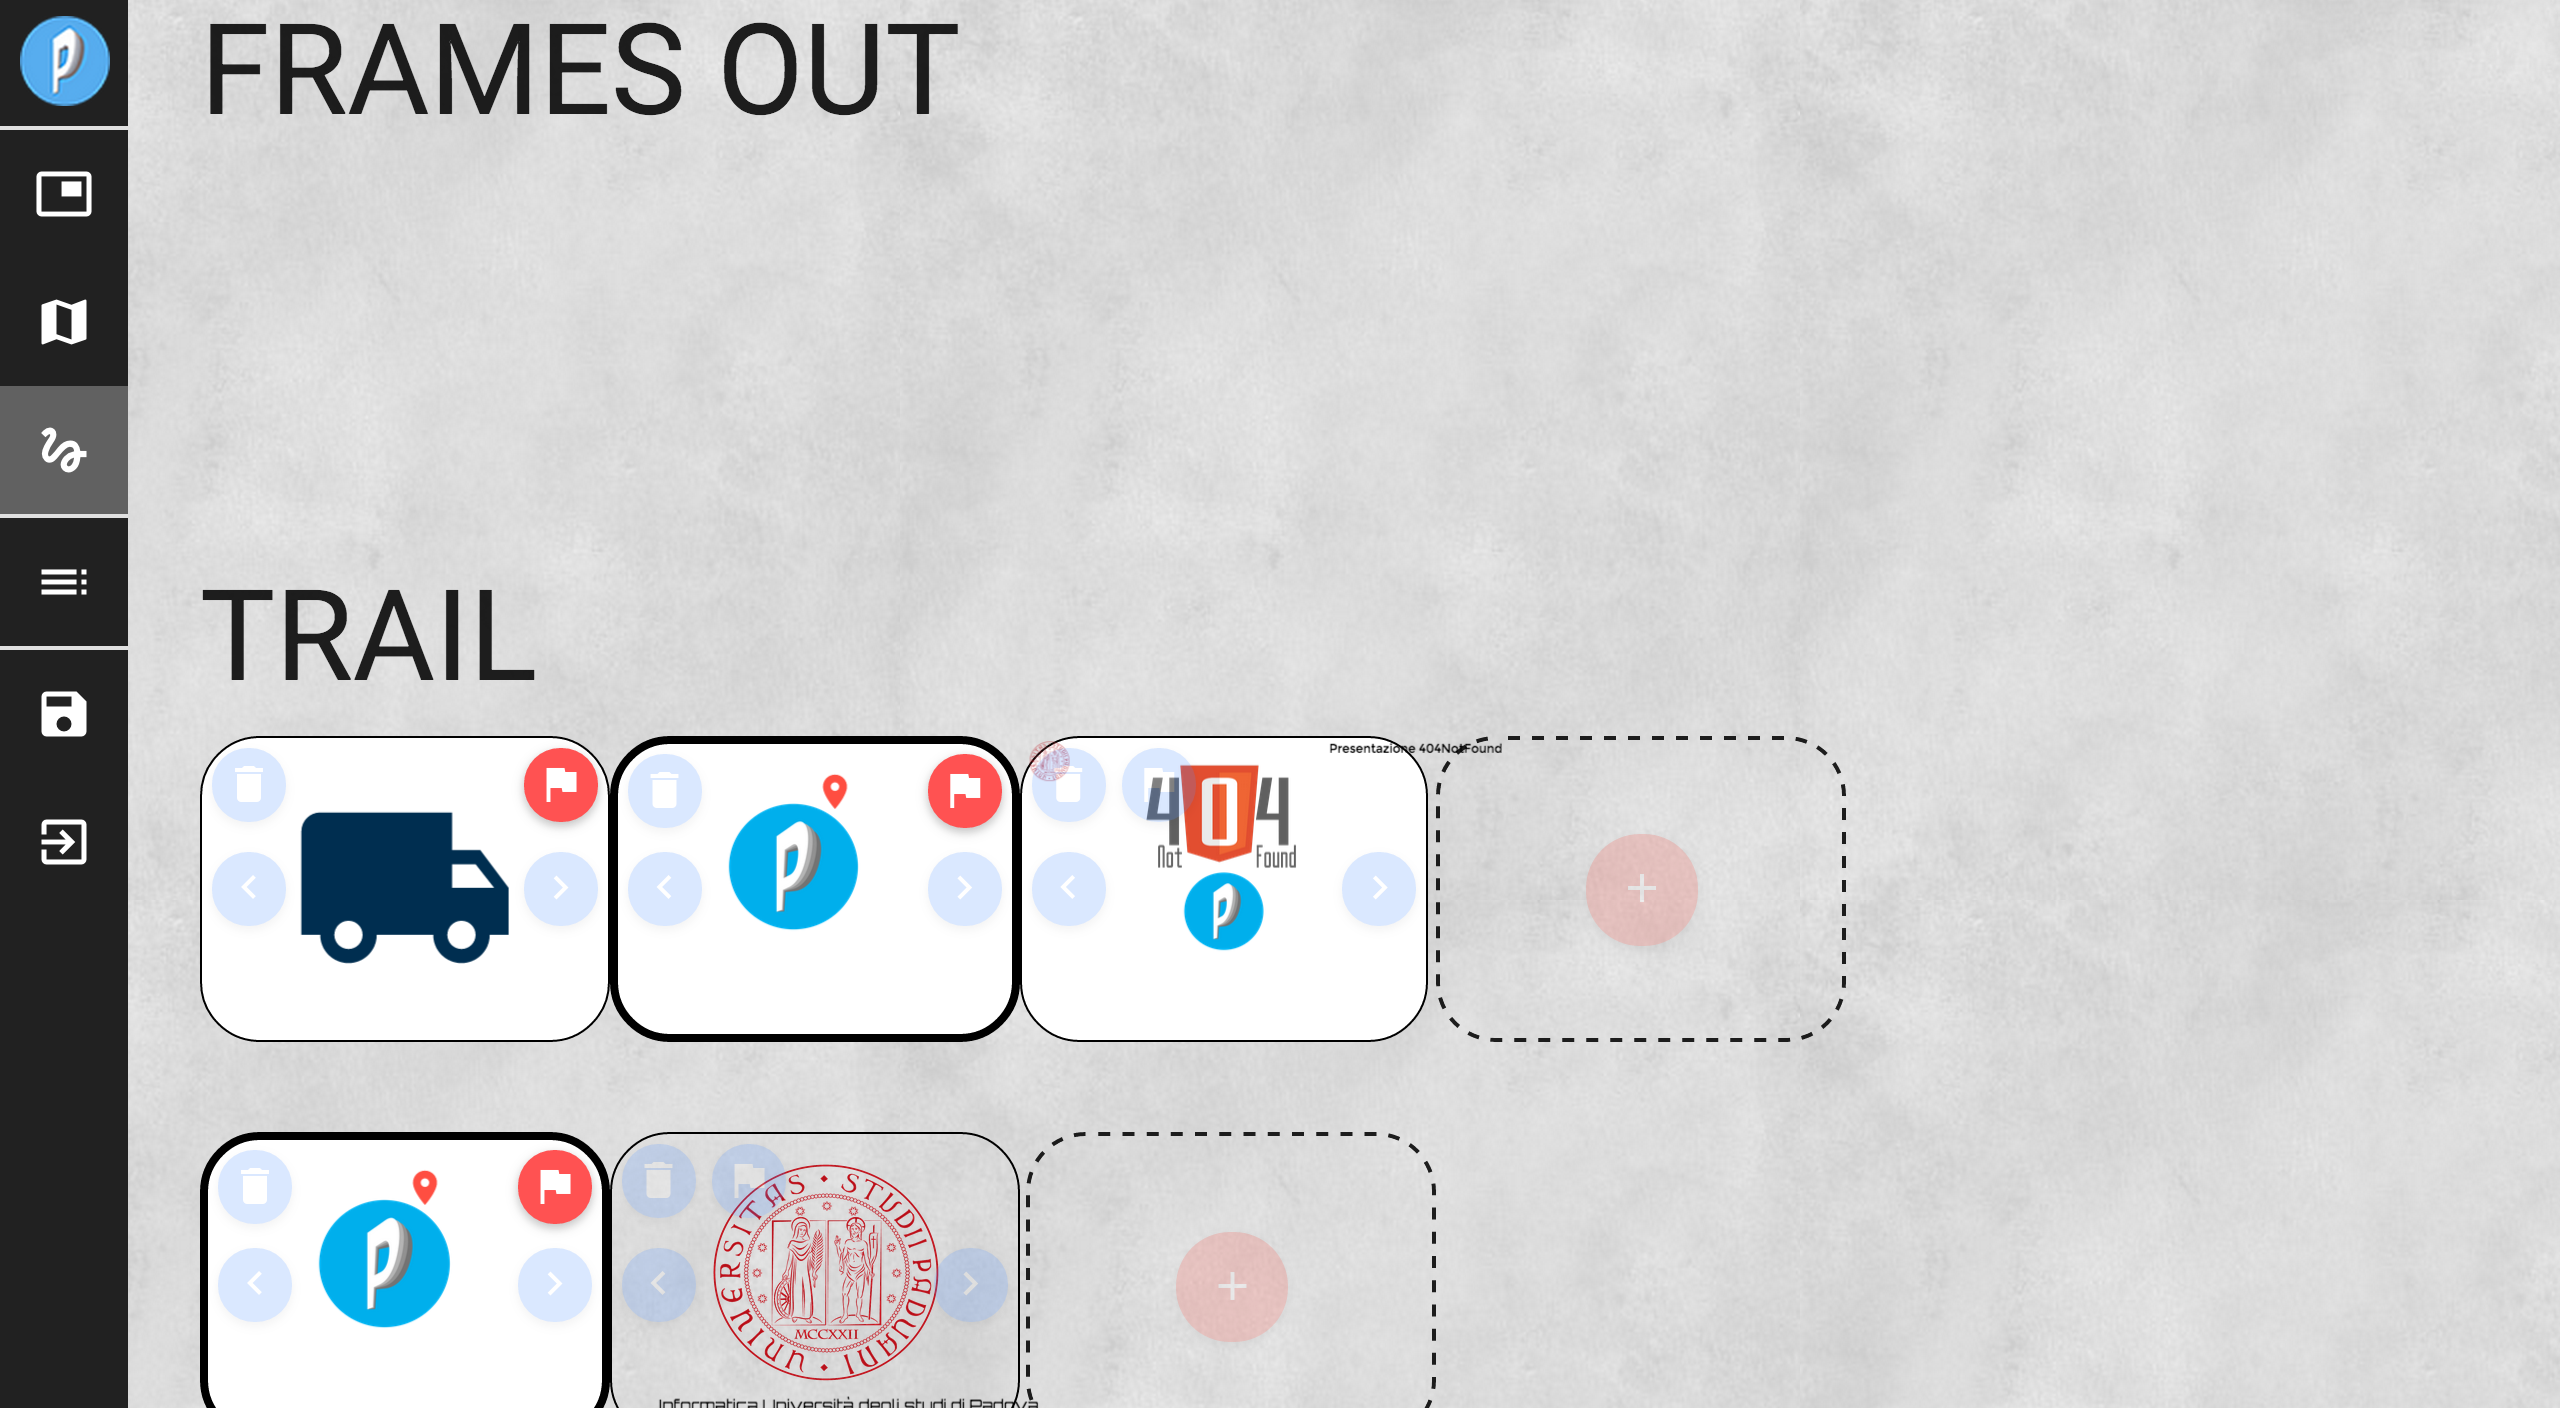
\includegraphics[scale=0.35]{img/trail_frame.png}
\caption{Modalità Trails editor$_G$.}
\end{center}
\end{figure}

\subsection{Avvio di una presentazione}
Per avviare una presentazione premere sul comando 
\includegraphics[scale=0.5]{img/play.png} della presentazione che si vuole avviare.\\

\begin{figure}[!h]
\begin{center}
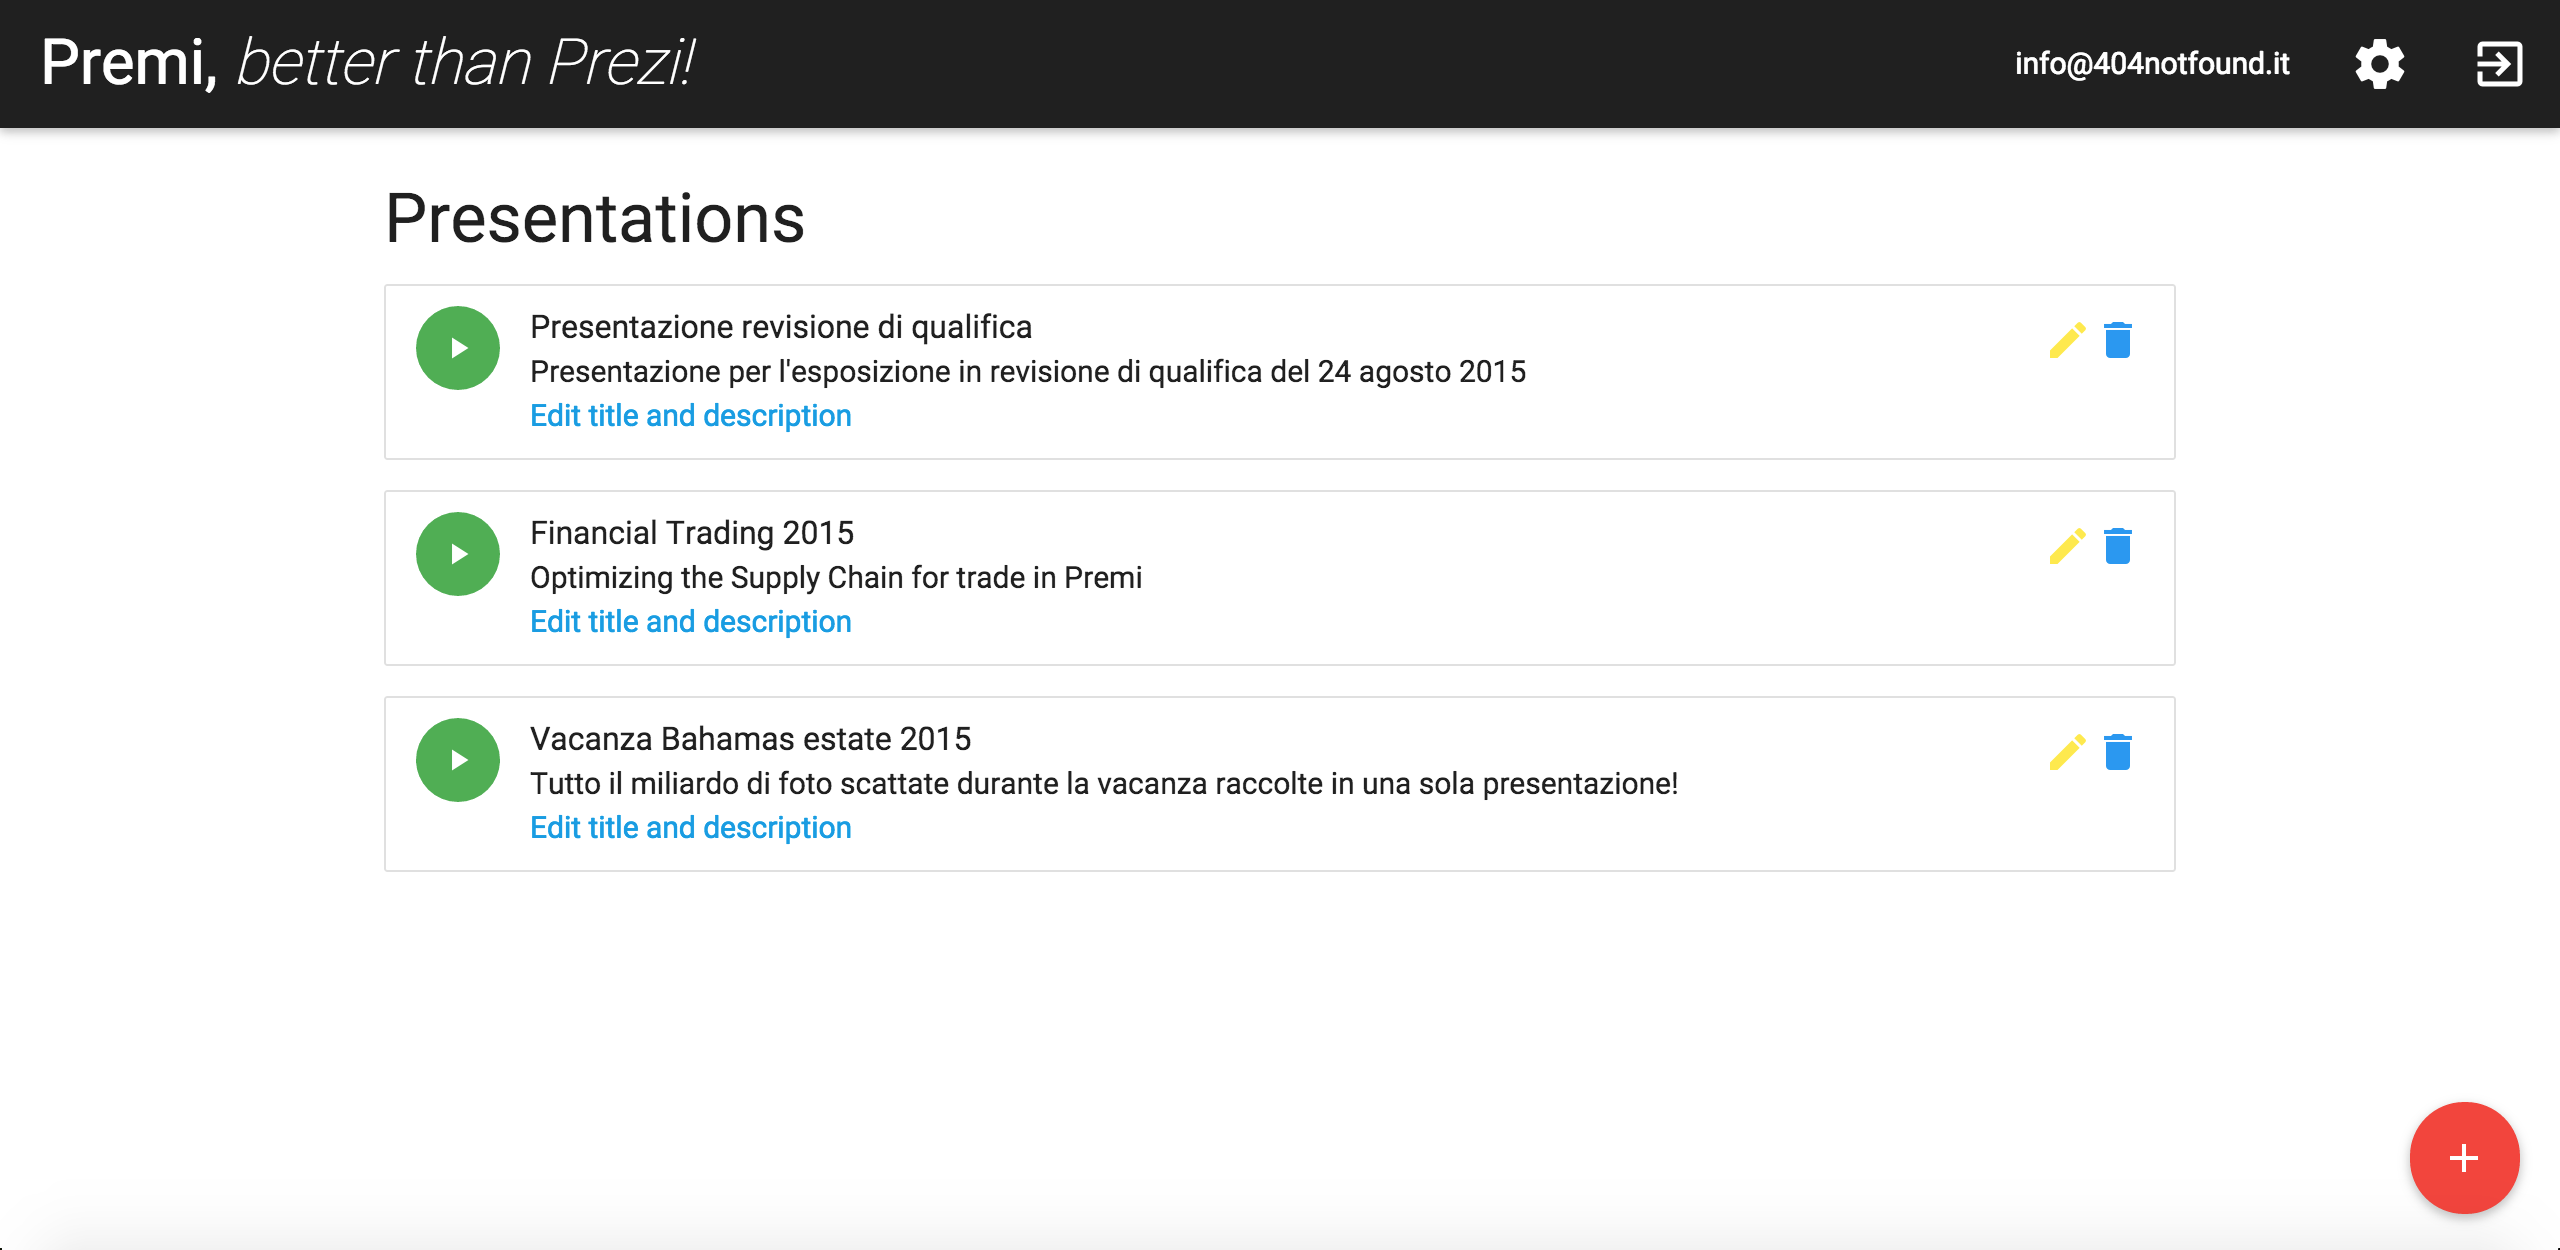
\includegraphics[scale=0.35]{img/dashboard.png}
\caption{Modalità Trails editor$_G$.}
\end{center}
\end{figure}

Verrà in seguito richiesto di selezionare uno dei trails creati da utilizzare per riprodurre la presentazione corrente. Selezionarlo, analogamente alla presentazione, con il comando 
\includegraphics[scale=0.5]{img/play.png}.\\
Si aprirà quindi il visualizzatore:

\begin{figure}[!h]
\begin{center}

\includegraphics[scale=0.3]{img/viewer.png}
\caption{Modalità Trails editor$_G$.}
\end{center}
\end{figure}

Dove i comandi sono:

\begin{tabular}{ c p{15cm}}
\parbox[c]{2em}{
\includegraphics[scale=0.4]{img/checkpoint2.png}} & Permette di tornare al checkpoint$_G$ precedente nel caso in cui ci si trovi in un percorso di approfondimento.\\
\parbox[c]{2em}{
\includegraphics[scale=0.4]{img/prev.png}} & Frame$_G$ precedente.\\
\parbox[c]{2em}{\includegraphics[scale=0.4]{img/next.png}} & Frame$_G$ successivo.\\
\parbox[c]{2em}{\includegraphics[scale=0.4]{img/down.png}} & Permette di spostarsi in un percorso di approfondimento ove presente.\\
\parbox[c]{2em}{\includegraphics[scale=0.4]{img/quit3.png}} & Uscita dal visualizzatore.
\end{tabular}

\subsection{Errori e loro cause}
Durante l'utilizzo dell'applicazione c'è la possibilità di imbattersi in alcuni errori, dovuti ad un uso scorretto dell'applicativo oppure ad alcune anomalie. Per quanto riguarda errori non previsti o malfunzionamenti dell'applicazione fare riferimento alla sezione 1.5 \emph{Come segnalare problemi e malfunzionamenti} del documento corrente.\\

Gli errori più comuni si possono riscontrare in sede di autenticazione, registrazione o cambio password e sono dovuti ad un inserimento non corretto dei dati richiesti.

\begin{figure}[!h]
\begin{center}
\includegraphics[scale=0.4]{img/signup_error.png}%
\qquad\qquad
\includegraphics[scale=0.4]{img/signup_error2.png}
\caption{Errori in fase di registrazione.}
\end{center}
\end{figure}

Tali errori possono essere evitati rispettando alcuni vincoli sui campi richiesti:
\begin{itemize}
\item \textbf{Email}: l'indirizzo email deve essere in un formato corretto, cioè \emph{nome@dominio.estensione} (Es. info@404notfound.it);
\item \textbf{Password}: il campo password non deve essere vuoto;
\item \textbf{Confirm password}: il campo di conferma password deve corrispondere alla password precedentemente inserita.
\end{itemize}
\newpage
Anche in fase di autenticazione si possono riscontrare errori simili.\\

\begin{figure}[!h]
\begin{center}
\includegraphics[scale=0.4]{img/signin_error.png}%
\qquad\qquad
\includegraphics[scale=0.3]{img/signin_error2.png}
\caption{Errori in fase di registrazione.}
\end{center}
\end{figure}

Vincoli necessari sui campi per l'autenticazione:
\begin{itemize}
\item \textbf{Email}: l'indirizzo email deve essere in un formato corretto, cioè \emph{nome@dominio.estensione} (Es. info@404notfound.it);
\item \textbf{Password}: il campo password non deve essere vuoto;
\item \textbf{Dati inseriti}: i dati inseriti devono corrispondere a quelli utilizzati in fase di registrazione.
\end{itemize}

Durante il cambio della password i vincoli sul campo password sono gli stessi visti in precedenza, mentre è possibile riscontrare un nuovo errore: \emph{Error changing password}.

\begin{figure}[h]
\begin{center}
\includegraphics[scale=0.35]{img/change_pass_error.png}
\caption{Errore cambio password.}
\end{center}
\end{figure}

Tale errore si presenta quando sul campo \emph{Old Password} viene inserita una password non corrispondente a quella corrente.
